\documentclass{article}
\usepackage[utf8]{inputenc}
\usepackage{soul}
\usepackage{graphicx}
\usepackage[margin=0.5in]{geometry}
\usepackage{color}
\usepackage{listings}
\usepackage{pdflscape}
\usepackage{afterpage}
\lstset{basicstyle=\footnotesize,breaklines=true}
\usepackage{url}
\usepackage{booktabs}
\usepackage{cleveref}
\usepackage{amsmath}
\newcommand\ie{i.\,e.\;}
\newcommand\etal{\textit{et al}.\;}
\newcommand{\todo}[1]{\textcolor{red}{\textbf{---TODO: #1}---}}
\begin{document}

\title{lucidML \\ Technical Documentation}
\author{Alan Schelten \and Lukas Galke \and Dennis Brunsch \and Florian Mai}
\maketitle
\tableofcontents
\newpage

\section{Introduction}
\subsection{Motivation}
Gro\ss{}e-B\"olting \etal \cite{grosse2015comparison} compared a number of methods
for automated semantic document annotation. Their framework is implemented
as a pipeline with four different major stages, wherein each stage can
be replaced with a different one to form a different method. This
document describes the technical details of \emph{LucidML}, a
Python-based framework that reflects the pipeline pattern's strengths in
terms of flexibility and (re-)implements some of the most successful methods for
automated semantic document annotation according to Gro\ss{}e-B\"olting \etal as
well as a number of new approaches. Those new approaches were chosen to work
well for the case when only the title of a document is available, as explored
in our paper \cite{quadflor}.
\subsection{Structure of Document}
In chapter \ref{applicationdesign} we describe the framework's architecture from
a high level point of view and show the stages'
functions and interfaces. We then list what methods are actually
implemented and how they can be combined.
In chapter \ref{implementation} we
explain the implementation itself, such as what parameters can be used.
In the appendix, we provide tutorials for installing and usage of
the command-line script as well as how one
should approach the code to extend it with new methods.

This document only covers the technical realization of the framework and its
included methods. It does not justify the choice of methods nor
evaluate them in any context.
For this, please read our paper \cite{quadflor}.
\section{Application Design}\label{applicationdesign}
\subsection{Architecture}
As shown in \Cref{fig:pipeline}, the pipeline consists of the steps
\emph{Input}, \emph{Feature Extraction}, \emph{Vectorization}, \emph{Reweighting}, \emph{Classification} and \emph{Evaluation}.

Given a corpus of input documents and an input thesaurus,
both are read and preprocessed in the \emph{Input} phase.
In the \emph{Vectorization} phase, features are then extracted either using terms or concept detection.
These are either used to build a graph for graph-based vectorization or the frequencies are counted.
Hierarchical spreading activation then can add further information using the hierarchical thesaurus.
When testing the model, the first two phases are executed for both the training and the test set,
since here each sample is considered separately.
The \emph{Reweighting} phase uses statistical reweighting methods to penalize very common features in the
document corpus.
In the subsequent \emph{Classification} step, classifiers are trained on the training set.
In the \emph{Evaluation} step that model is used to predict labels for the samples in the test set.
By comparing those labels to the true labels we know from the gold standard, those
predictions are then used to estimate the quality of the model according to a
some metrics.
\subsection{Input}
\begin{itemize}
  \item input: File paths
  \item output: Preprocessed documents and thesaurus.
\end{itemize}
The documents and thesaurus are tokenized, lemmatized and stop-words are removed.

\subsection{Feature Extraction}
\begin{itemize}
  \item input: preprocessed documents
  \item output: documents with extracted features.
\end{itemize}
In this step, all documents in the corpus are processed to extract \emph{features}.
What is considered as a feature is determined by some policy which one has to configure for this step.
In our case features can either be single words in the document, concepts or synsets.
Single words are extracted using a regular expression.
Concepts are detected by matching series of words in the document to a domain-specific thesaurus.
Synsets are detected using WordNet and Lesk Word Sense Disambiguation.


\subsection{Vectorization}
\begin{itemize}
  \item input: documents containing only extracted features
  \item output: feature matrix, containing one feature vector per document
\end{itemize}
The detected features' values are determined by either considering their cooccurences with other features or by their
raw frequency count.

The cooccurences are used to create a graph for graph-based activation.

The frequency counts can be changed by applying hierarchical spreading activation,
which adds further information using the hierarchical thesaurus.
\subsection{Reweighting}
\begin{itemize}
  \item input: feature vectors from the training set
  \item output: reweighted feature vector
\end{itemize}
This step takes the feature vectors of all documents in the training set and uses this information
to calculate a factor for each feature which depends on
the frequency of a feature in the complete corpus.
This is then used to change the values of the training and test set.

\subsection{Classification}
\begin{itemize}
  \item input: a partition of the feature vectors into test- and training set
  and the gold standard
  \item output: a classification model and a set of labels per document in the
  test set
\end{itemize}
In the fashion of a typical machine learning classification task, the
feature vectors of the training set are used to learn a \emph{classifier},
which maps feature vectors onto a set of labels.
The \emph{gold standard} is used for training.
By applying that mapping to the test set, we get a set of labels per document in the test set.
A classifier may be subject additional input, such as estimation
 parameters or the raw document input.
\subsection{Evaluation}
\begin{itemize}
  \item input: a set of predicted labels and a set of true labels per document
  in the test set
  \item output: a collection of values
\end{itemize}
Here, a number of metrics are applied to estimate the quality of the model
learned in the previous step.
In addition to the predicted labels and the true
labels, a metric may also consider external information, such as relations
between labels.

\subsection{Methods}
Although the structure of the output in the previous steps is fixed, the
concrete values heavily depend on the methods/metrics used. Subsequently, we
list the methods that have been implemented and where they were introduced in
the literature.
\begin{itemize}
  \item Feature extraction
  \begin{itemize}
    \item Synset Extraction: Uses WordNet \cite{wordnet} and Lesk's algorithm \cite{Lesk:1986:ASD:318723.318728}.
    \item Concept Extraction: See Große-Bölting \etal \cite{grosse2015comparison}.
  \end{itemize}
  \item Statistical activation methods
	\begin{itemize}
    \item TF-IDF: See Salton \etal \cite{salton1988term}.
    \item BM25: See Robertson \etal \cite{robertson1999okapi}.
  \end{itemize}
  \item Graph-based activation methods
  \begin{itemize}
    \item Degree
    \item Betweenness: See Freeman \cite{freeman77}.
    \item Closeness Centrality: See Bavelas \cite{bavelas50}.
    \item Katz centrality: See Katz \cite{katz53}.
    \item HITS: See Zouaq \etal \cite{zouaq2012voting}.
    \item PageRank: See Page \etal \cite{page1999pagerank}.
  \end{itemize}
  \item Hierarchical activation methods
  \begin{itemize}
    \item Basic: See Anderson \etal \cite{anderson83}.
    \item Children: Own Development
    \item OneHop: See Große-Bölting \etal \cite{grosse2015comparison}.
    \item BellLog: See Kapanipathi \etal \cite{kapanipathi14}.
    \item Bell: See Kapanipathi \etal \cite{kapanipathi14}.
    \item HCF-IDF: See Nishioka \etal \cite{nishioka2015influence}.
  \end{itemize}
  \item Classifiers
  \begin{itemize}
    \item kNN-based classifiers
    \begin{itemize}
      \item BR-KNNa/b: See Spyromitros \etal \cite{spyromitros2008empirical}
      \item 1NN
    \end{itemize}
    \item Linear support vector machine
    \item Logistic Regression
    \item Stochastic Gradient Descent using log-loss (estimating Logistic Regression)
    \item Stacked Classifier: See Hess \etal \cite{hess2008multi}.
      In Contrast to Hess, we use Stochastic Gradient Descent as well as Rocchio
      with log-loss as a bass classifier and
      Decision Trees as a meta-classifier.
    \item Rocchio Classifier: See Sebastiani \cite{sebastiani2002machine}.
  \end{itemize}
  \item Evaluation metrics
  \begin{itemize}
    \item Label-based Macro-F1
    \item Label-based Micro-F1
    \item Label-based Macro-Recall
    \item Label-based Macro-Recall
    \item Label-based Micro-Precision
    \item Label-based Micro-Precision
    \item Document based F1
    \item Document based Recall
    \item Document based Precision
    \item Hierarchical F1-measure: See Kiritchenko \etal \cite{Kiritchenko04familihierarchical}.
  \end{itemize}
\end{itemize}

\subsection{Combining pipes/methods}
Figure \ref{fig:pipeline} displays methods that have been realized.
\begin{figure}[thb!]
    \centering
    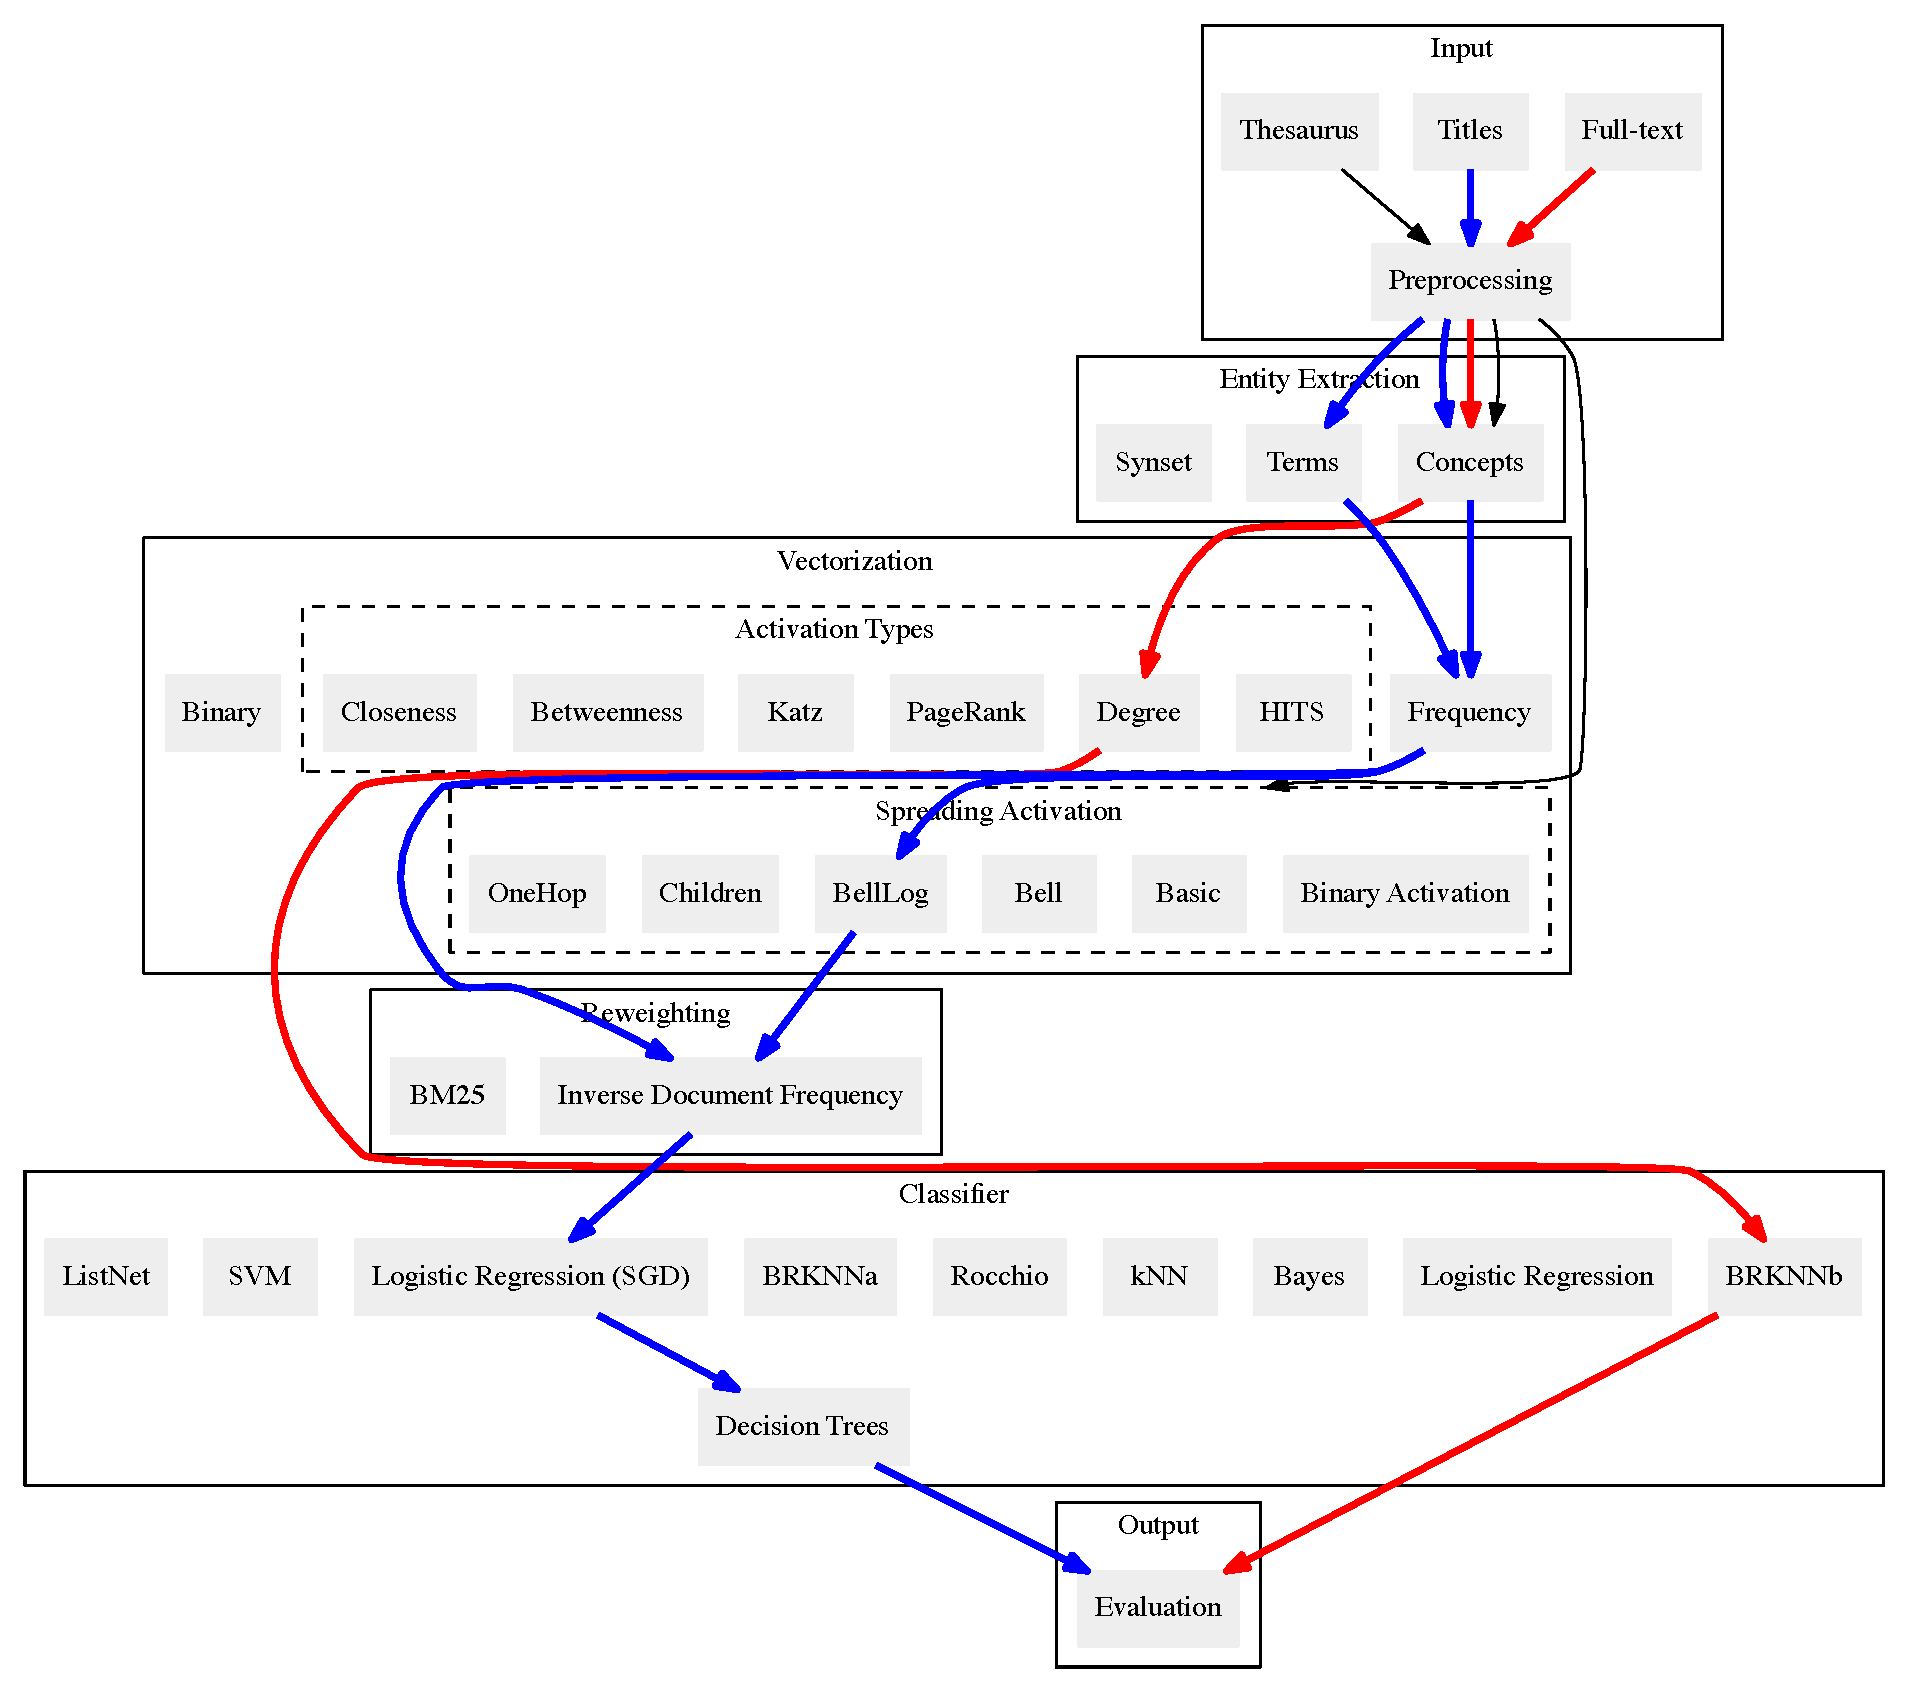
\includegraphics[width=\textwidth]{graphics/pipelineExtended.pdf}
    \caption{
      Illustration of the configurable text processing pipeline.
      The emphasized edges and nodes show two example configurations.
      The red edges correspond to the configuration: \texttt{-F -cg degree -f brknnb}.
      The blue edges correspond to: \texttt{-ctbH belllog -f sgddt}.
      The black lines show the use of the thesaurus.
    }
    \label{fig:pipeline}
  \end{figure}

\section{Implementation}\label{implementation}
  \subsection{Scikit-Learn}
The pipeline structure described above was implemented in Python 3. The implementation
uses methods of the Python package \textit{scikit-learn} (also referred to as \textit{sk-learn}),
which provides an extensive set of tools for
data mining and machine learning \cite{scikit-learn}. In the context of
scikit-learn a pipeline sequentially applies a list of \textit{transformations} (corresponding
to some parts of the preprocessing, the extraction phase, and activation phase) and a
final \textit{estimator} (corresponding to
the classification phase). A transformer provides the methods \texttt{fit} and \texttt{transform}
whereas an estimator provides the methods \texttt{fit} and \texttt{predict}. Obviously, in case of classification,
which is the way we use it, an estimator provides the same functionality as commonly known from a classifier in machine
learning. The fit methods translates to the training of the classifier and the predict method translates to
the prediciton of classes for unseen samples.

The methods provided
by scikit-learn operate on the data given as a matrix where each row
represents a \textit{sample} (in our application, that is the full text or the title of a document) and
each column represents a \textit{feature} (in our application, that is a term or a concept detected in a
document).

For an extensive introduction to scikit-learn, please refer to their tutorial section\footnote{The tutorial section can be
found at \url{http://scikit-learn.org/stable/tutorial/}}.

In order to conform with the pipeline structure of scikit-learn, we made heavy use of the transformers available
for NLP applications, as well as the large variety of estimators available. Furthermore, in those cases where the
functionality we required has not been included in the framework, we created new estimators from scratch or modified
existing estimators to serve our purpose. Specifically, we created the classes \texttt{SpreadingActivationTransformer}, \texttt{GraphVectorizer},
and \texttt{BM25Transformer} as transformers. We created \texttt{RocchioClassifier}, \texttt{ClassifierStack}, \texttt{NearestNeighbor},
\texttt{KNeighborsListNetClassifier}, and \texttt{BRKNeighborsClassifier} as estimators.
\subsection{The Main class}
The main script of our implementation is called \texttt{run.py} and implements the main aspects of the
abstract pipeline structure mentioned above. It consists of seven main sections:

\begin{itemize}
  \item loading and preprocessing the data
  \item extracting features
  \item choosing the scoring method
  \item building the classifier
  \item configuring the pipeline
  \item cross validation
  \item evaluation
\end{itemize}

In the following paragraphs we will discuss the implementation details of some of these sections.
The overall structure is determined by the options available.


\subsection{Loading and preprocessing the data}

\subsubsection{Extractor}
The method for loading the data is called \texttt{load\textunderscore data} which is implemented in lucid\textunderscore \texttt{ml/utils/Extractor.py}.
The data (documents as strings - \texttt{X\textunderscore raw}, gold standard as list of strings - \texttt{Y\textunderscore raw})
is given as a python dictionary of the form \texttt{<document\textunderscore id>: <data>} and the thesaurus as a \texttt{ThesaurusReader}.
The data is given as two lists (\texttt{X\textunderscore raw}, \texttt{Y\textunderscore raw}) where the indexes
are unique in the sense that \texttt{X\textunderscore raw[i]=s} and \texttt{Y\textunderscore raw[i]=l} if and only if the gold standard represented by
\texttt{l} is associated with the document represented by \texttt{s} and identified by \texttt{i}.

When testing configurations or running the script locally, it can be a good idea to reduce the size of the input data.
This can be done using the \texttt{{-}{-}toy} option.
For example \texttt{{-}{-}toy 0.1} uses 10\% of the input data.

\subsubsection{Preprocessing}
Preprocessing is handled by the \texttt{NltkNormalizer} class.
As the name suggests, it makes heavy use of the nltk library\footnote{
  \url{http://www.nltk.org/}, accessed 03/30/2016.
}.
Preprocessing is not handled as a separate step, instead this class centrally offers
methods which are used in several places in the code.
Note that it is not recommendable to use the nltk methods such as \texttt{lemmatize} directly,
because this loads the lemmatizer from disk on each call,
which slows down the processing significantly.
Instead the \texttt{NltkNormalizer} loads all necessary resources on initialization or lazily as needed.

The preprocessing follows the following steps:
First the input is tokenized, then stop-words are removed and the remaining words lemmatized using \texttt{nltk.WordNetLemmatizer}.
The tokenization is done using a custom regular expression: \texttt{r"(?u)\textbackslash b[a-zA-Z\_][a-zA-Z\_]+\textbackslash b"}
accepts all words of alphabetic characters with length 2 or longer.
Note that this excludes numbers.

\subsubsection{Persister}
When using the persist option (\texttt{-p}) the data loading, feature extraction and scoring steps are saved to disk
and reloaded when using the same configuration and the same data using the \texttt{Persister} class.
This leads to significantly faster execution times, when comparing different classifiers.
The extracted concepts are saved separately.
Changes in the time stamps of the files or different configurations lead to the steps being re-executed and saved again.
If the concept extraction method is not changed and the files stay the same,
the concepts are not re-calculated for differing configurations.
The folder for persisting the files can be set using the \texttt{{-}{-}persist\_to} option and
recalculating and saving the features can be forced using the option \texttt{{-}{-}repersist}.
Although the class tries to clean up old files, it can leave garbage behind.
This has to be cleaned up manually.

\subsection{Extracting and counting features}
In any case, we use SK-Learns CountVectorizer class\footnote{
  \url{http://scikit-learn.org/stable/modules/generated/sklearn.feature_extraction.text.CountVectorizer.html},
  accessed 03/30/2016. }
to count the frequencies of the features in a document. By using the 'analyzer' parameter, the
CountVectorizer can either be passed a function that identifies a feature or one of the pre-defined options for feature detection. In our application,
we use the following call to the constructor in order to extract single terms:
\begin{lstlisting}[language=Python]
terms = CountVectorizer(input=input_format, stop_words='english', binary=options.binary,
                        token_pattern=word_regexp)
\end{lstlisting}
The option \texttt{input\_format} corresponds to the option \texttt{-F},
telling the CountVectorizer whether to expect a file object or a list of filenames to open.
\texttt{stop\_words} activates the standard scikit-learn stop-word list.\footnote{
  See \url{https://github.com/scikit-learn/scikit-learn/blob/master/sklearn/feature_extraction/stop_words.py}, accessed 03/28/2016.
}
The words in this list are removed from the input data.
The binary option (\texttt{-b}) reduces the counted words to binary vectors.
This can be interesting when using very little data, such as titles.
\texttt{word\_regexp} refers to the regular expression defined in the \texttt{NltkNormalizer} which tokenizes the input.

For the concept extraction, however, we created the \texttt{ConceptAnalyzer} class.
The concept extraction works in principle as described by Große-Bölting \cite{boltingMaster2015} in Chapter 6.3.1.1.
At each position in the string of the document or title,
the following words are compared to the thesaurus.
In the case of finding more than one match in the thesaurus,
the entry with the longest match is chosen.
The only difference to the description by Große-Bölting is that number of words which are compared to
the thesaurus corresponds to the maximal number of words of a label in the thesaurus.
The \texttt{ConceptAnalyzer} offers an \texttt{analyze} method which can be passed to the
\texttt{CountVectorizer} using the \texttt{analyzer} keyword argument.

As an alternative feature extraction method, you can try using the \texttt{SynsetAnalyzer}.
Similar to the concept extraction described above, this class offers an \texttt{analyze}
method which can be passed to the \texttt{CountVectorizer}.
The \texttt{SynsetAnalyzer} uses WordNet \cite{wordnet} to try to detect a synset for each word.
A synset tries to capture the meaning of a group of synonyms.
Since each word can be part of a group of synsets,
the correct synset is estimated using the Lesk word sense disambiguation algorithm \cite{Lesk:1986:ASD:318723.318728}.
The class is implemented using the nltk library.

When we want to use a graph-based scoring, we use a slightly different extraction method, because we need to count cooccurences of terms.
This is realized in the
GraphVectorizer class, which is also a Transformer in the sense of scikit-learn.
If the option \texttt{-c} is set, the graph is built using concepts extracted as described above.
Otherwise, it uses terms.
See \Cref{subsubsec:graphbased} for a more detailed description.

\subsection{Scoring - Weighting - Reweighting}
As graph-based scoring is fundamentally different from statistical scoring due to different inputs, we will examine them differently in the following subsections.
\subsubsection{Statistical and Hierarchical Methods}
For the statistical methods, we always count how often a feature appears in a document first. Given the frequency,
we can optionally apply one of the spreading activation methods and one of the reweighting methods.

\paragraph{Reweighting methods}
As reweighting methods, one can choose from \emph{TF-IDF} and \emph{BM25}. For the exact definitions of either of them, please
refer to our paper. For TF-IDF reweighting we used SK-Learns TfIdfTransformer class \footnote{
  see \url{http://scikit-learn.org/stable/modules/generated/sklearn.feature_extraction.text.TfidfTransformer.html}, accessed 04/16/2016.
}.
The BM25 reweighting is done by the BM25Transformer class, which is an adaption to Python 3 of an open-source
implementation of BM25. By default we only use the parameters that fit our definition given in the paper, but
if you would like to configure it differently, please refer to the original files
\footnote{The original file can be found at \url{https://gist.github.com/psorianom/0b9d8a742fe0efe0fe82}}.
\paragraph{Spreading activation methods}
For the spreading activation method, one can choose from one of the following:
'basic', 'bell', 'belllog', 'children', 'binary', 'onehop'.
BellLog and OneHop are discussed in detail in our paper.
The generic definition of spreading activation reweighting is given by the following equation for a concept $i$ in a document $d$:
\begin{align}
	\operatorname{score}_\text{sa}(i,d) = \operatorname{score}(i) + \lambda \sum_j w(i,j) \operatorname{score}_\text{sa}(j)
	\label{eq:sa}
\end{align}
Where the concepts $j$ are connected by weighted edges $w(i,j)$ to the concept $i$.
In case of using a semantic thesaurus resembling a hierarchy of concepts, the edges are typically given by the
narrower edges of the thesaurus (or parent-child relations).
The spreading activation method 'basic' corresponds to setting $w(i,j) = 1 \forall i,j$
and adjusting $\lambda$ as a hyperparameter.

The spreading activation methods 'bell' and 'belllog' scale down the $\operatorname{score}_\text{sa}$
by the number of concepts on the next level or the logarithm, respectively.
This can be achieved by setting the weights of the edges in the generic definition as follows:
\begin{align*}
	w(i,j) &= \frac{1}{\operatorname{levelcount}(j)} &\tag{bell}\\
	w(i,j) &= \log_{10} \frac{1}{\operatorname{levelcount}(j)} &\tag{belllog}
	\label{}
\end{align*}
where $\operatorname{levelcount}(j)$ gives the number of concepts in the same level as $j$.
Note that in a \emph{polyhierarchy}, the definition with $\operatorname{levelcount}(j)$
differs from using $\operatorname{levelcount}(i+1)$ of the next level in the hierarchy
as weighting factor for all child nodes.
This is caused by the possible occurences of \emph{child} nodes, that are still on a \emph{higher}
level in the hierarchy.
Assuming that such structures appear at the bottom of the hierarchy, 'bell' and 'belllog' would actually be undefined
for the $i+1$ variant, but are defined by using the level count of the target child node ($j$ variant).
The alternative would be pruning the polyhierarchy to a tree,
so that the two variants would be equivalent.
But this resulted (pruning performed in a breadth first manner) in more than 50\% removed edges
in one of our datasets (econBiz), corresponding to a undesirably big information loss.

\emph{The devil lies in the (implementation) details.
\footnote{German saying which basically means that details need to be considered carefully.}}
Straightforward implementing Equation \ref{eq:sa} results in a recursive computation,
which has to be performed for each single document in the corpus.
Even with memoization techniques, this is computationally not affordable.
Therefore, the spreading activation is typically performed bottom-up.
The score value of a concept $j$ is added to all its parent's $i$ score values,
scaled by the decay parameter $\lambda$ the edge weight $w(i,j)$ (this process is called \emph{firing}).
In order to preserve the ideas of early spreading activation approaches,
and to be able to limit the spreading at some point, we also provide
a firing threshold as hyperparameter. The concepts only fire when this firing threshold is exceeded.
Still, we mostly set this hyperparameter to zero
to retain the original behavior of 'bell' and 'belllog' spreading activation methods.
Additionally, the concepts are restricted to firing only once.

%%% MARKER PASSING
\emph{Marker passing} is a technique to implement spreading activation efficiently.
We maintain a queue of index markers, which node exceeds the firing threshold and therefore
activates its predecessors.
When one of these predecessors' new score exceeds the firing threshold $F$ (usually $F=0$),
its index is added to the queue.

\begin{lstlisting}[language=python]
# input matrix X
# I -- document indices
# J -- feature (concept) indices
# V -- values
# hierarchy -- the underlying hierarchy, given by a thesaurus
# F -- firing threshold
# fired -- indicator matrix for the nodes already fired
# markers -- queue of markers (i,j-pairs) for firing candidates
# output matrix X_out
I, J, V = sp.find(X) # find nonzero entries
X_out[I,J] = V # copy to output
markers = deque(zip(I,J)) # initialize marker queue
while markers:
    i, j = markers.popleft()
    if X_out[i,j] >= F and not fired[i,j]:
	fired[i,j] = True
	for target in hierarchy.predecessors(j):
	    X_out[i,target] += X_out[i,j] * decay * hierarchy[target][j]['weight'] # activate

	    if X_out[i, target] >= F:
		markers.append((i,target)) # pass the marker, if threshold exceeded

\end{lstlisting}
This technique allows to implement all variants of the generic spreading activation definition.
The spreading activation methods 'basic', 'bell', 'belllog', and 'children' can be implemented by
preprocessing the edge weights of the hierarchy accordingly.
The huge benefit of this technique is, that the whole feature matrix can be processed simultaneously
by starting with its non-zero entries and continuing by passing the markers.
Therefore, we do \emph{not} need to traverse the whole hierarchy for each single document at a time.

The spreading activation method 'binary' was created for binary (occurence) data instead of count data.
It differs from the other methods by performing the logical $\operatorname{or}$ among the children of a node.
This results in setting the whole path (to the root) of all extracted concepts in a document to one,
which emphasizes the similarity of documents even in scenarios with very few extracted concepts.
This can also conveniently performed on the whole feature matrix simultaneously,
by starting at its non-zero entries and setting all ancestors to $1$.

The spreading activation method 'onehop' performs a single pass over the feature matrix,
activating the concepts that have more than 2 non-zero child concepts.
The score of a parent concept $i$ with child concepts $j$ is given by $\frac{1}{\lambda} \sum_j \operatorname{score}$,
when there are more than 2 non-zero child concepts, and $\operatorname{score}$ else.
The implementation can also be performed simultaneously on the whole feature matrix as follows.
Since 'onehop' spreading activation explicitly performs only one pass,
we do not need to pass markers.
To maintain generality we parametrize the spreading activation method by the threshold of activated child concepts,
and the decay parameter $\lambda$, which is usually set to $0.4$.
\begin{lstlisting}[language=python]
# X -- input feature matrix
# I -- document indices
# J -- feature (concept) indices
# threshold -- threshold for number of activated child concepts
# X_out -- output feature matrix
I, J, _ = sp.find(X)
for i, j in zip(I,J):
    n_children = 0
    sum_children = 0
    for child in hierarchy.successors(j):
	if X[i, child] > 0: # same row i
	    n_children += 1
	    sum_children += X[i, child]
    if n_children >= threshold:
	X_out[i,j] = X[i,j] + sum_children * decay
    else:
	X_out[i,j] = X[i,j]
\end{lstlisting}

\subsubsection{Graph based Methods}
\label{subsubsec:graphbased}
Graph based Methods construct the graph by creating edges for each neighboring feature.
These are directed for the method \texttt{'hits', 'pagerank', 'katz'}
and undirected for all other methods.
The implementation of the graph scoring algorithms is delegated to the \texttt{networkx} package.
For documentation of the algorithms used, see the \texttt{networkx} documentation.\footnote{
\url{https://networkx.github.io/documentation/latest/reference/algorithms.html}, accessed 03/28/2016.}

\subsection{Classification}
\paragraph{Building the classifier}
Building the classifier mainly depends on the option \texttt{-f}, \texttt{{-}{-}classifier},
which provides a key corresponding to one of several classifiers.
The hyperparameters of these classifiers are partly pre-configured and can be partly further customized by further options.
\begin{description}
  \item[\texttt{nn}, \texttt{brknna}, \texttt{brknnb}, \texttt{mcknn}, \texttt{rocchio}, \texttt{listnet}]
    These keys correspond to the 1-Nearest-Neighbor classifier,
    the binary relevance KNN classifiers (in variants a and b),
    the mean-cut KNN classifier,
    the Rocchio (nearest centroid) classifier,
    and the ListNet K-neighbors classifier.
    The distance metric used is the cosine distance,
    which requires the brute-force algorithm.
    The number of neighbors $k$ considered is controlled by the options \texttt{-n}.
    For the first three classifiers (\texttt{nn}, \texttt{brknna}, \texttt{brknnb}),
    it is possible to enable auto-optimizing $k$ paremeter by setting the option \texttt{-G, {-}{-}grid-search}.
    As the computational cost of computing the distances to all examples of the training set may become expensive,
    the option \texttt{-l,{-}{-}lshf} enables an approximation
    of the nearest neighbors by locality sensitive hashing forests.
  \item[\texttt{mbayes}, \texttt{bbayes}]
    These two keys are used to access the Multinomial Naive Bayes and Bernoulli Naive Bayes classifiers.
    The multi-label support is supplied by the one vs rest scheme.
    Their smoothing parameter $\alpha$ can be contolled by the option \texttt{-a, {-}{-}alpha}.
  \item[\texttt{lscv}, \texttt{logregress}]
    The key \texttt{lsvc} corresponds to a linear support vector classifier,
    and \texttt{logregress} corresponds to a logistic regression classifier.
  \item[\texttt{sgd}]
    This key corresponds to the averaged stochastic gradient descent classifier with logistic loss.
    Many hyperparameters can be customized by the options:
    \texttt{-e, {-}{-}epochs} defines the number of sweeps over the dataset,
    \texttt{-P, {-}{-}penalty} specifies the penalty term on the weights (l1,l2,elasticnet), and
    \texttt{-a, {-}{-}alpha} specifies the $\alpha$ parameter, which is used as a factor for the penalty term,
    and is also used to compute the learning rates.
  \item[\texttt{sgddt}, \texttt{rocchiodt}, \texttt{logregressdt}]
    are the keys corresponding to the ClassifierStack approach with a decision tree as meta classifier
    and \texttt{sgd}, \texttt{rocchio} or \texttt{logregress} as base classifiers.
\end{description}

Some of the following classifiers are not by default enabled for multi-labeling,
namely both Naive Bayes classifiers, Linear SVC, Logistic Regression and
Stochastic Gradient Descent (SGD). In order to obtain a multi-label-classifier, we use Scikit-Learn's OneVsRestClassifier
and feed it an indicator matrix\footnote{
\url{http://scikit-learn.org/stable/modules/generated/sklearn.multiclass.OneVsRestClassifier.html#sklearn.multiclass.OneVsRestClassifier}, accessed 03/28/2016.}.
The OvR method learns a binary classifier for each label. As these classifiers are trained independent of
each other, the procedure can be heavily parallelized by passing the classifier the number of concurrent
jobs with the n\_jobs parameter.
\paragraph{BatchKNeighbors for kNN-based classifiers}
The scikit-learn package implements the search for nearest neighbors without taking memory problems into account,
by calculating the pairwise distances of each testing sample to each training sample and saving this matrix to memory.
This can lead to memory problems for datasets with many samples.
\texttt{BatchKNeighbors} solves this by splitting the test set into batches.
The size of the batch can be set by defining the approximate maximum amount of memory to be used in GB when calling the
\texttt{kneighbors} method with the \texttt{approx\_max\_ram\_GB} keyword argument.
When initializing, the class is passed an object which implements a \texttt{kneighbors} method such as
\texttt{LSHForest} or \texttt{NearestNeighbors} from scikit-learn.
\paragraph{NearestNeighbor}
The \texttt{NearestNeighbor} classifier is discussed in detail in our paper.
It is called in \texttt{run.py} as:
\begin{lstlisting}[language=Python]
NearestNeighbor(use_lsh_forest=options.lshf)
\end{lstlisting}

\texttt{use\_lsh\_forest} chooses whether to use scikit-learns LSHForest implementation.\footnote{
  \url{http://scikit-learn.org/stable/modules/generated/sklearn.neighbors.LSHForest.html}, accessed 03/28/2016.
}
This approximates the nearest neighbor and in theory is less memory intensive and faster.
In practice however, it performed much worse in both regards when setting the parameters in such a way,
so that the success of the method was comparable.

\paragraph{BRkNN-a and BRkNN-b}
\texttt{BRKNeighborsClassifier} implements the BRkNN algorithms as specified by Spyromitros \etal \cite{spyromitros2008empirical}:
\begin{lstlisting}[language=Python]
 BRKNeighborsClassifier(mode='a', n_neighbors=options.k, use_lsh_forest=options.lshf, algorithm='brute', metric='cosine', auto_optimize_k=options.grid_search)
 \end{lstlisting}
The \texttt{auto\_optimize\_k},  \texttt{n\_neighbor\_candidates} and \texttt{scoring} keyword arguments control the auto-optimization of k.
This is not implemented using scikit-learns \texttt{GridSearch} because it's implementation at version 0.17 did
not accept the input for $Y$ (the labels) as a sparse matrix.
This prevented some datasets to fit into memory.

\texttt{use\_lsh\_forest} works as described above.
\paragraph{KNeighborsListNet}
The class KNeighborsListNetClassifier is a procedure mainly inspired by Huang \etal \cite{huang2011recommending},
where the authors used ListNET to rank all the labels that occur among the n-nearest neighbors.

To this end, for each of the labels appearing in the neighborhood, they extracted a set of features using the documents
in the neighborhood. A training sample used for the training of the ranking method then consists of the set of features of the label
and the binary indication whether the label is assigned to the document in question.
Finally, for new samples, the k highest ranked labels are assigned as output.

Not all parts of the procedure as introduced by Huang \etal can readily be applied to our application. Hence, some of the
features generated differ slightly.
The features that are generated are the following:
\begin{itemize}
  \item the sum of the cosine similarities to all the documents in the n-neighborhood that the label is actually assigned to
  \item the total count of appearances of the label in the document
  \item the probability that the label translates to the document's title according to the IBM1-translation-model\footnote{
  \url{https://en.wikipedia.org/wiki/IBM_alignment_models}}.
  \item the count of how often the label directly appears in the title
\end{itemize}
This algorithm uses the ListNET implementation from
RankLib\footnote{For the source code please refer to the projects page at \url{https://sourceforge.net/p/lemur/wiki/RankLib/}}
in the background. Hence, it assumes a Java-
installation to be available and the RankLib-2.5.jar file to be in the same folder as this file.
\paragraph{Bernoulli Naive Bayes and Multinomial Naive Bayes}
We used Scikit-Learn's implementation\footnote{\url{http://scikit-learn.org/stable/modules/naive_bayes.html}} for both qualifiers.
Both can be given an $\alpha$ value to be used for Lidstone-Smoothing, which can be specified via the '-a' option of the run script.
\paragraph{Linear SVC}
Again, we realized the linear SVC using the Scikit-Learn implementation. You can specify a relatively large number of
hyperparameters, like the penalty parameter $C$, the loss function, the loss-metric and some more. As the
classifier takes very long to be trained when the number of labels and features is large (on a machine with 24 cores, it took
roughly 3 days on the Economics dataset's full-text which has more than 2 million features and more than 6000 labels),
the default hyperparameters given are by no means optimized.
\paragraph{Logistic Regression}
Due to similar reasons as for the linear SVC, training this classifier takes a long time. Again, the hyperparameters
as we chose them are not reliablty optimized either.
However, we found that, among all powers of two, choosing $C = 64$ in the Scikit-Learn implementation \footnote{\url{http://scikit-learn.org/stable/modules/generated/sklearn.linear_model.LogisticRegression.html}}
obtains reasonably good results (see \ref{sec:extended_results}).
\paragraph{Stochastic Gradient Descent (SGD)}
The scikit-learn implementation of SGD \footnote{\url{http://scikit-learn.org/stable/modules/sgd.html}} lets you specify one of the pre-defined loss function to approximate,
which can obtain very good results with relatively low computational cost:
The mathematical formulation and the chosen hyperparameter values are described in detail in our paper \cite{quadflor}.
\begin{lstlisting}[language=Python]
sgd = OneVsRestClassifier(SGDClassifier(loss='log', n_iter=options.max_iterations, penalty=options.penalty, alpha=options.alpha, average=True),
        n_jobs=options.jobs)
\end{lstlisting}
In our implementation, we used the \emph{log-loss} to obtain the behavior of
Logistic Regression. By specifying \emph{loss='squared\_hinge'}, however, a linear SVC
is obtained. The default parameters we use were manually optimized for the Economics dataset and those
worked decently well on the other datasets, too.
Averaging the weights over time results in faster convergence and allows higher learning rates.
The rather low $\alpha$-value of $10^-7$ implies rather low (l2-)regularization and rather high initial learning rates
according to the default learning rate update schedule 'optimal' of scikit-learn.
We favor the logarithmic loss over the squared hinge loss, since it results in equal or even better performance
in terms of the 'f1\_samples'-metric on our datasets (especially the Economics dataset) and enables predicting probabilities,
so that SGD can be used as a base classifier for the multi-value stacking approach.

\paragraph{Rocchio}
In our paper, we explain how we adapted Rocchio for the multi-label-case and how we can compute a probability that a sample
belongs to a class. Instead of cosine distance, one can also define euclidean to be the distance measure.
Furthermore, our Rocchio-implementation requires a fix number $k$ as input. After training, a new sample is assigned
the $k$ top classes that yield the highest probability.

To fit the multi-label case, we modified scikit-learn's NearestCentroid class
\footnote{\url{http://scikit-learn.org/stable/modules/generated/sklearn.neighbors.NearestCentroid.html}} accordingly.
\paragraph{RocchioDT, SGDDT, and LogRegressDT}
The ClassifierStack class is an implementation of Multi-Value-Stacking procedure described in detail in our paper:
\begin{lstlisting}[language=Python]
ClassifierStack(base_classifier=sgd, n_jobs=options.jobs, n=options.k)
\end{lstlisting}
It must be provided with a base classifier that is expected to have a \emph{fit} and a \emph{predict\_proba} function at least.
The predict\_proba function is a scikit-learn specific function that returns a probability of a sample belonging to each of the
possible labels. These probabilties are considered to be the confidence values.
You can also specify the number of parallel jobs executed when generating the training samples for the meta classifier. This is
the most expensive operation of the classifier computation-wise, so you probably want to make use of that option.
The parameter $n$ determines the size of the top-list of most confident labels. Per training sample, the computational cost increases
linearily with it. Trying to improve the choice of $n$ manually, we found that $n = 10$ already gives reasonably good results and slightly
improves around 30. If $n$ becomes too large, the performance decreases. We believe that this is due to noise being added to the
meta-classifiers' training sets.
As meta-classifier we use the Decision Tree implementation from Scikit-Learn
\footnote{\url{http://scikit-learn.org/stable/modules/generated/sklearn.tree.DecisionTreeClassifier.html#sklearn.tree.DecisionTreeClassifier}}.

\subsection{Cross validation}
For the evaluation of the computed classification we use $k$-fold cross validation. That means, the data set is split into $k$
(\texttt{options.folds}) smaller sets, called folds. Then, for each fold $F$ the remaining $k-1$ folds are used to train a model
and $F$ is used to validate the model. We use the implementation provided by scikit-learn
namely the classes \texttt{KFold}\footnote{
  \url{http://scikit-learn.org/stable/modules/generated/sklearn.cross_validation.KFold.html}, accessed 04/04/2016.}
(\texttt{options.cross\_validation==True}) and \texttt{ShuffleSplit}\footnote{
  \url{http://scikit-learn.org/stable/modules/generated/sklearn.cross_validation.ShuffleSplit.html}, accessed 04/04/2016}
(\texttt{options.cross\_validation==False}). The class \texttt{KFold} creates folds of equal sizes if possible. The class \texttt{ShuffleSplit}
creates a user defined number of independent data set splits in train and test data. The samples are first shuffled.
Both classes return train and test indices to split the data set in train and test sets.
We compute different metrics for each set using methods provided by scikit-learn and numpy. In \Cref{metrics},
we describe the used metrics and their application in detail.

\subsection{Metrics}\label{metrics}
In this section, we describe the metrics we used for evaluation and how they are implemented in lucidML. For the implementation, we used methods
provided by scikit-learn\footnote{
  \url{http://scikit-learn.org/stable/modules/classes.html#sklearn-metrics-metrics}, accessed 04/04/2016}, numpy\footnote{
  \url{http://www.numpy.org/}, accessed 04/04/2016} and scipy\footnote{
  \url{https://www.scipy.org/}, accessed 04/04/2016}.
For the following paragraphs, we fix a set of labels $L$, a document corpus $D$ and a classifier $\gamma$. We write $\mathrm{gold}(d)$ to denote the
gold standard of a document $d$. We also need some preliminary definitions. First, let
\begin{equation*}
\mathrm{precision}(A,B) = \frac{|A \cap B|}{|A|},
\qquad
\mathrm{recall}(A,B) = \frac{|A \cap B|}{|B|},
\end{equation*}
\begin{equation*}
\mathrm{F}(A,B) = \frac{2 \cdot \mathrm{precision}(A,B) \cdot \mathrm{recall}(A,B)}{\mathrm{precision}(A,B) + \mathrm{recall}(A,B)},
\end{equation*}
for arbitrary sets $A$ and $B$. In the implementation of scikit-learn, it holds that $\mathrm{precision}(A,B) = 0$ if $A = \emptyset$ and similar for
$\mathrm{recall}$ and $\mathrm{F}$. Furthermore, we will talk about true and false positives (tp and fp) and false negatives (fn) which are defined as
\begin{equation*}
\mathrm{tp}(d) = | \{l \in L | l \in \gamma(d), l \in \mathrm{gold}(d) \}|,
\end{equation*}
\begin{equation*}
\mathrm{fp}(d) = | \{l \in L | l \in \gamma(d), l \notin \mathrm{gold}(d) \}|,
\end{equation*}
\begin{equation*}
\mathrm{fn}(d) = | \{l \in L | l \notin \gamma(d), l \in \mathrm{gold}(d) \}|.
\end{equation*}
Finally, we need to talk about the predictions of $\gamma$. Therefore, we define the sets of predicted pairs $\mathrm{T}$ and true predicted
pairs $\overline{\mathrm{T}}$
\begin{equation*}
\mathrm{T} = \{(d,l) | d \in D, l \in \gamma(d) \},
\qquad
\overline{\mathrm{T}} = \{(d,l) | d \in D, l \in \gamma(d), l \in \mathrm{gold}(d) \},
\end{equation*}
as well as the sets of predicted and true predicted pairs relative to some document $d$ or label $l$
\begin{equation*}
\mathrm{T}_{d} = \{(d',l) \in y | d'=d \},
\qquad
\mathrm{T}_{l} = \{(d,l') \in y | l'=l \}.
\end{equation*}
Similarly, the sets $\overline{\mathrm{T}}_{d}$ and $\overline{\mathrm{T}}_{l}$ are defined.

\paragraph{Sample-based F1}
For each document $d$, the F1 score is defined as
\begin{equation*}
\mathrm{F1}(d) =  \mathrm{F}(\mathrm{precision}(\gamma(d),\mathrm{gold}(d)),\mathrm{recall}(\gamma(d),\mathrm{gold}(d)))
\end{equation*}
It is a value in $[0,1]$. The sample-based F1 measure is the average of the F1 scores of all documents in the test corpus
\begin{equation*}
\frac{1}{|D|} \sum\limits_{d \in D} \mathrm{F}(\mathrm{T}_{d},\overline{\mathrm{T}}_{d}).
\end{equation*}
We used the method \texttt{f1\_score}\footnote{
  \url{http://scikit-learn.org/stable/modules/generated/sklearn.metrics.f1_score.html}, accessed 04/07/2016} provided by scikit-learn
to compute the sample-based F1 measure.

\paragraph{Sample-based Precision}
The precision of $\gamma$ for some document $d$ is defined as
\begin{equation*}
\frac{\mathrm{tp}(d)}{\mathrm{tp}(d) + \mathrm{fp}(d)}
\end{equation*}
It is a value in $[0,1]$ and denotes the ability of $\gamma$ not to consider a sample as positive when it is negative. The sample-based
precision is the average of the precision scores of all documents in the test corpus
\begin{equation*}
\frac{1}{|D|} \sum\limits_{d \in D} \mathrm{precision}(\mathrm{T}_{d},\overline{\mathrm{T}}_{d}).
\end{equation*}
We used the method \texttt{precision\_score}\footnote{
  \url{http://scikit-learn.org/stable/modules/generated/sklearn.metrics.precision_score.html}, accessed 04/07/2016} provided by scikit-learn
to compute the sample-based precision.

\paragraph{Sample-based Recall}
The recall of $\gamma$ for some document $d$ is defined as
\begin{equation*}
\frac{\mathrm{tp}(d)}{\mathrm{tp}(d) + \mathrm{fn}(d)},
\end{equation*}
The recall score is a value in $[0,1]$ and denotes the ability of $\gamma$ to find all positive samples. The sample-based recall is the average of
the recall scores of all documents in the test corpus
\begin{equation*}
\frac{1}{|D|} \sum\limits_{d \in D} \mathrm{recall}(\mathrm{T}_{d},\overline{\mathrm{T}}_{d}).
\end{equation*}
We used the method \texttt{recall\_score}\footnote{
  \url{http://scikit-learn.org/stable/modules/generated/sklearn.metrics.precision_score.html}, accessed 04/07/2016} provided by scikit-learn
to compute the sample-based recall.

\paragraph{Macro- and Micro-Average}
The macro- and micro-average F1 measures are then defined as follows
\begin{equation*}
\textrm{macro-F1} : \frac{1}{|L|} \sum\limits_{l \in L} \mathrm{F}(\mathrm{T}_{l},\overline{\mathrm{T}}_{l}),
\qquad
\textrm{micro-F1} : \mathrm{F}(\mathrm{T},\overline{\mathrm{T}}).
\end{equation*}
The macro- and micro-average precision and recall are defined as
\begin{equation*}
\textrm{macro-precision} : \frac{1}{|L|} \sum\limits_{l \in L} \mathrm{precision}(\mathrm{T}_{l},\overline{\mathrm{T}}_{l}),
\qquad
\textrm{micro-precision} : \mathrm{precision}(\mathrm{T},\overline{\mathrm{T}}),
\end{equation*}
\begin{equation*}
\textrm{macro-recall} : \frac{1}{|L|} \sum\limits_{l \in L} \mathrm{recall}(\mathrm{T}_{l},\overline{\mathrm{T}}_{l}),
\qquad
\textrm{micro-recall} : \mathrm{recall}(\mathrm{T},\overline{\mathrm{T}}).
\end{equation*}

\paragraph{Average number of labels}
We also compute the average number of predicted labels per document (\texttt{avg\_n\_labels\_pred} and \texttt{avg\_n\_labels\_gold})
using methods provided by numpy.

\paragraph{Hierarchical F1 measure}
Using the \texttt{-r} option enables the evaluation of the hierarchical F-1 measure.
Using this measure is only possible if (1) the thesaurus actually contains hierarchical references
and (2) the labels in the gold standard are a subset of the labels in the thesaurus.

The hierarchical F1-measure implemented was developed by Kiritchenko \etal \cite{Kiritchenko04familihierarchical}
and is defined as the harmonic mean of hierarchical precision and hierarchical recall.
These are defined as follows:
Let $\mathrm{C}_\mathrm{t}$ represent the set true classes of and example and $\mathrm{C}_\mathrm{p}$ the predicted classes.
Moreover, let $\mathrm{ancestor}(C)$ be the set containing $C$ and all it's ancestors in the hierarchy,
excluding the root node.
Then the hierarchical precision $\mathrm{hP}$ is:
\[\mathrm{hP} = \frac{\vert \mathrm{ancestor}(\mathrm{C}_\mathrm{p}) \cap \mathrm{ancestor}(\mathrm{C}_\mathrm{t})\vert}{\vert \mathrm{ancestor}(\mathrm{C}_\mathrm{p})\vert}\]

And the hierarchical recall $\mathrm{hR}$ is:
\[\mathrm{hR} = \frac{\vert \mathrm{ancestor}(\mathrm{C}_\mathrm{p}) \cap \mathrm{ancestor}(\mathrm{C}_\mathrm{t})\vert}{\vert \mathrm{ancestor}(\mathrm{C}_\mathrm{t})\vert}\]
The hierarchical F1 measure is implemented in \texttt{utils.metrics}.

\subsection{Examples}
To sequence diagram in figure \ref{fig:example} correspondes to the configuration \texttt{-F -cg degree -f brknnb} illustrated
by the red arrows in figure \ref{fig:pipeline}. It shows the main steps processed by lucidML. For completion, we will describe where
to find the scripts and classes occuring in the sequence diagram:
\begin{itemize}
  \item \texttt{lucid\_ml.run.py}
  \item \texttt{lucid\_ml.utils.Extractor.py}
  \item \texttt{lucid\_ml.utils.thesaurus\_reader.ThesaurusReader}
  \item \texttt{lucid\_ml.weighting.concept\_analysis.ConceptAnalyzer}
  \item \texttt{lucid\_ml.weighting.graph\_score\_vectorizer.GraphVectorizer}
  \item \texttt{lucid\_ml.classifying.br\_kneighbor\_classifier.BRKNeighborsClassifier}
  \item \texttt{sklearn.pipeline.py}\footnote{
    \url{http://scikit-learn.org/stable/modules/generated/sklearn.pipeline.Pipeline.html}, accessed 04/08/2016.}
  \item \texttt{sklearn.cross\_validation.ShuffleSplit}\footnote{
    \url{http://scikit-learn.org/stable/modules/generated/sklearn.cross_validation.ShuffleSplit.html}, accessed 04/08/2016.}
 \end{itemize}

\begin{figure}[hbt!]
    \centering
    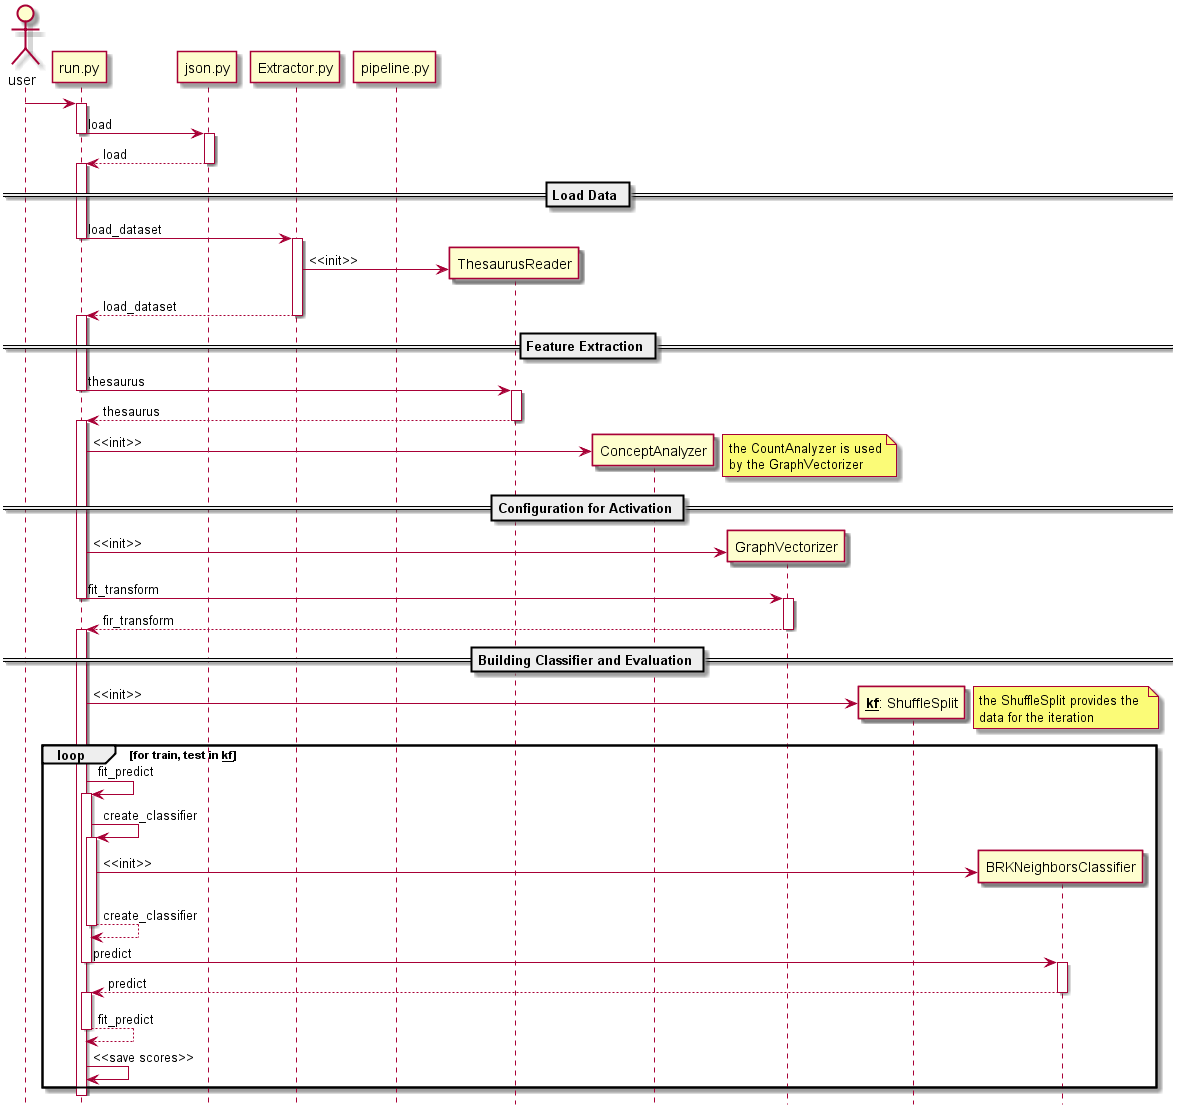
\includegraphics[width=\textwidth]{graphics/sequence_DEGREE_BRKNNB.png}
    \caption{
      Illustration of the configuration: \texttt{-F -cg degree -f brknnb}.
    }
    \label{fig:example}
\end{figure}

\section{Appendix}
\subsection{Tutorials}
In these tutorials, you will be shown how to run experiments on your local machine, configure the pipeline via the command line, and how to implement new
pipes for the pipeline and integrate them within the framework.
\subsubsection{Installation guide}
To avoid unnecessary overhead in the documentation, we will assume that your local machine is a Linux distribution and, more specifically, Ubuntu 14.04.
However, the required tools are available for all common systems, so you will be able to easily apply these steps to your favorite system as well,
assuming that you have some proficiency in googleing\footnote{\url{https://en.wikipedia.org/wiki/Google_(verb)}}.

The framework is written in Python 3. Although the code might also run with lower versions, we recommend installing Python 3.4 or higher.
Before we get started with python, you will need to install a few other libraries. Simply run:
\begin{lstlisting}[basicstyle=\ttfamily]
$ sudo apt-get install libatlas-base-dev gfortran python3.4-dev python3.4-venv build-essential
\end{lstlisting}
Now to python!
Pip is a tool that lets you install the required modules in a convenient fashion.
venv lets you create virtual environments for your Python installation with helps to avoid trouble when
working on multiple Python projects on the same machine. In the command line, run:
\begin{lstlisting}[basicstyle=\ttfamily]
$ python3 -m venv lucid_ml_environment
\end{lstlisting}
This creates a directory that contains a python3.4 executable and all the default packages, including pip. By running the command
\begin{lstlisting}[basicstyle=\ttfamily]
$ source lucid_ml_environment/bin/activate
\end{lstlisting}
you can activate the environment, which basically prepends all the necessary paths  to your PATH-environment-variable temporarily.
Hence, running \emph{python} should now execute the instance of Python 3.4 in your \emph{lucid\_ml\_environment} directory. You
can deactivate it with the \emph{deactivate} command.

Having activated the environment, you need to install the packages required. As said before, pip is a convenient tool to achieve that.
Conveniently, all python requirements are listed in the requirements.txt located at the base folder of the project.
Run:
\begin{lstlisting}[basicstyle=\ttfamily]
  $ cd Code
  $ pip install -r requirements.txt
\end{lstlisting}
This may take a while. Have you had your daily dose of coffee or tea yet? This is probably a good opportunity to get more!
\subsubsection{How to use the command line tool}
First of all, activate the virtual environment that you set up in the previous step, so you're running a python version that comes with all the necessary requirements.
All experiments can be run by executing the run.py script with the parameters set accordingly. Consider the following example, which runs CTF-IDF
with the 1NN classifier on the example dataset which is provided with the code: Assuming you're in the root-directory of the project's repository within a bash-shell,
execute the following:
\begin{lstlisting}[basicstyle=\ttfamily]
$ cd Code/lucid_ml
$ python run.py -c -t -f nn -k file_paths.json -K example-titles -x
\end{lstlisting}
As it's common in command-line based tools, parameter options to the script are indicated with the prefix '-'. Typically, an option is
abbreviated by a single character, like 'c', 't' and 'f' in this example, but it isn't mandatory. The order of the options' appearance does not matter.
You may also put multiple options after a single '-' character.
\begin{lstlisting}[basicstyle=\ttfamily]
$ python run.py -ctxf nn -k file_paths.json -K example-titles
\end{lstlisting}
However, some options come with an additional value indicated by an '=' symbol or a whitespace, like 'f', 'k', 'K' and '{-}{-}toy'.

The options used in this example are the most critical ones and will be used often. So what do they do exactly?

'K' and 'k' determine
the dataset that will be used in the experiment. With 'k' you provide the script with the relative or absolute path to a file that itself contains the paths
to the datasets. That file must have JSON format and maps a key to a relative or absolute path. The key used is what is given by the 'K' option. In our example,
'file\_paths.json' is located in the 'Code/lucid\_ml' directory and contains the paths to the example dataset (including text, goldstandard and thesaurus) that
are located within the repository. Hence,
if you are implementing new stuff and want to test it we recommend doing so locally on your computer given the keys above. Please consider that the
datasets are typically very large. Hence, depending on how much memory your machine has, you may want to run the code with only a fraction of the data,
which you can specify with the '{-}{-}toy' option. Typically, when working with the Economics title dataset examined in our paper~\cite{quadflor},
25\% of the data should already give you a good measure of how well your new method performs and should still not exceed 4GB of RAM.

When your dataset is such that each document is contained in an individual file where the file's name has the form \emph{$<$identifier$>$.txt}, in the file\_paths.json you need to specify the path
to the directory that contains these files. In order to let the script know it is given file-based documents, you have to specify this with the '-F' switch like in our example:

\begin{lstlisting}[basicstyle=\ttfamily]
$ python run.py -ctxf nn -k file_paths.json -K example-fulltext -F
\end{lstlisting}

The classifier used in the experiment is specified by a key passed to the 'f' option. When 'c' and 't' are passed to the script, terms and extracted concepts will both be used
as features. 'x' means that a single-fold experiment is run, whereas 'X' will execute a full 10-fold-crossvalidation. These are only the most important features and there are many
more options available to tweak the algorithm, all of which are given
in \Cref{subsubsec:optionsoverview}.
This usage information can also be viewed by using the \texttt{-h} option as is common with command line tools.

As already mentioned, the procedure explained above will be what you want to execute during development,
parameter tweaking or quick evaluation of a single method. If you would like to run multiple experiments, however,
you would not like to need to start the next experiment after another has finished by hand. Instead, you can create a
configurations-file and run it like this:
\begin{lstlisting}[basicstyle=\ttfamily]
$ python run.py -C configurations_test.txt -x -o results.csv -k file_paths.json -K example-titles
\end{lstlisting}
The '-C' option is given the relative path to the configurations file, which looks like this:
 \begin{lstlisting}[language={}]
### evaluate tf-idf vs cf-idf
-c -f nn
-t -f nn
\end{lstlisting}
Each line in this file is interpreted as an experiment (except for the ones prefixed with \#, which denote comments).
Before running the experiment, all parameters given in the original call to the python script are appended to the list
of parameters passed to each experiment. In our example, the two experiments given equate to these two independent calls to
the run.py script:
\begin{lstlisting}[basicstyle=\ttfamily]
$ python run.py -c -f nn -x -o results.csv -k file_paths.json -K example-titles
$ python run.py -t -f nn -x -o results.csv -k file_paths.json -K example-titles
\end{lstlisting}
The '-o' option specifies the relative path to a file, to which the results of an experiment shall be written.
If the file doesn't exist, a new one is created. If it does exist, the results are appended to the end of it.
% \begin{table}[tb]
%     \centering
%     \caption{The options available to pass to the 'run.py' script.}
%     \label{tab:options}
%     \begin{tabular}{@{}c|c|c@{}}
%       \toprule
%       Option & Parameter & Description\\
%       \midrule
%         '-k', '{-}{-}key-file' & path to file & Specify the file to use as Key file for -K
%     \end{tabular}
% \end{table}
\subsubsection{Overview of all Options}
\label{subsubsec:optionsoverview}
\begin{lstlisting}[basicstyle=\ttfamily]
Optional Arguments
  -h, --help            show this help message and exit
  -C CONFIG_FILE, --config-file CONFIG_FILE
                        Specify a config file containing lines of execution
                        arguments
  -d, --dry             Do nothing but validate command line and config file
                        parameters
  -j JOBS               Number of jobs (processes) to use when something can
                        be parallelized. -1 means as many as possible.
  -o OUTPUT_FILE, --output OUTPUT_FILE
                        Specify the file name to save the result in. Default:
                        [None]
  -v, --verbose         Specify verbosity level -v for 1, -vv for 2, ... [0]
  --debug               Enables debug mode. Makes fit_predict method
                        debuggable by not starting a single fold in a new
                        process.
  -x                    Run on one fold [False]
  -X                    Perform cross validation [False]
  -i, --interactive     Use whole supplied data as training set and classify
                        new inputs from STDIN

  -r                    Calculate hierarchical f-measure (Only usable
  --worst WORST         Output given number of top badly performing samples by
                        f1_measure.

Detailed Execution Options:
  --test-size TEST_SIZE
                        Desired relative size for the test set [0.1]
  --folds FOLDS         Number of folds used for cross validation [10]
  --toy TOY_SIZE        Eventually use a smaller block of the data set from
                        the very beginning. [1.0]
  --training-error      Compute training error

Dataset Options:
  -F, --fulltext        Fulltext instead of titles
  -k KEY_FILE, --key-file KEY_FILE
                        Specify the file to use as Key file for -K
  -K DATA_KEY, --datakey DATA_KEY
                        Prestored key of data.

Feature Options:
  -c, --concepts        use concepts [False]
  -t, --terms           use terms [True]
  -s, --synsets         use synsets [False]
  -g {degree,betweenness,pagerank,hits,closeness,katz}, --graphscoring {degree,betweenness,pagerank,hits,closeness,katz}
                        Use graphscoring method instead of concepts and/or
                        terms
  --prune               Prune polyhierarchy to tree
  -H {basic,bell,belllog,children,binary,onehop}
                        Perform spreading activation.
  -B, --bm25            Use BM25 instead of TFIDF for final feature
                        transformation
  -b, --binary          do not count the words but only store their prevalence
                        in a document
  --no-idf              Do not use IDF
  --no-norm             Do not normalize values

Classifier Options:
  -f {nn,brknna,brknnb,bbayes,mbayes,lsvc,sgd,sgddt,rocchio,rocchiodt,logregress,logregressdt,listnet}, --classifier {nn,brknna,brknnb,bbayes,mbayes,lsvc,sgd,sgddt,rocchio,rocchiodt,logregress,logregressdt,listnet}
                        Specify the final classifier.
  -a ALPHA, --alpha ALPHA
                        Specify alpha parameter for stochastic gradient
                        descent
  -n K                  Specify k for knn-based classifiers. Also used as the
                        count of meta-classifiers considered for each sample
                        in multi value stacking approaches [1]
  -l, --lshf            Approximate nearest neighbors using locality sensitive
                        hashing forests
  -L n_components, --LSA n_components
                        Use Latent Semantic Analysis / Truncated Singular
                        Value Decomposition with n_components output
                        dimensions
  -G, --grid-search     Performs Grid search to find optimal K
  -e MAX_ITERATIONS     Determine the number of epochs for the training of
                        several classifiers [5]
  -P {l1,l2,elasticnet}
                        Penalty term for SGD and other regularized linear
                        models

Feature Persistence Options:
  -p                    Use persisted count vectors or persist if has changed.
  --repersist           Persisted features will be recalculated and
                        overwritten.
  --persist_to PERSIST_TO
                        Path to persist files.
\end{lstlisting}


\subsubsection{How to integrate a new classifier}
Say, you would like to integrate a new classifer into the framework, which simply assigns the $k$ most frequent labels.
As you already know, all steps in the
pipeline are transformers or - as the final step - an estimator. Each pipe is realized as its own class. So let's
create a new file \emph{stupid\_classifier.py} in the \emph{classifying} folder and put this code:
\begin{lstlisting}[language={Python}]
from sklearn.base import BaseEstimator
from scipy.sparse import csr_matrix
import numpy as np

class StupidClassifier(BaseEstimator):

    def __init__(self, k):
        self.k = k

    def fit(self, X, y):
        self.y = y
        frequencies = y.getnnz(axis = 0)
        self.most_frequent_labels = frequencies.argsort()[-self.k:][::-1]

    def predict(self, X):
        predictions = np.zeros((X.shape[0], self.y.shape[1]))
        for i in self.most_frequent_labels:
            predictions[:,i] = 1

        return csr_matrix(predictions)
\end{lstlisting}
Recall that an estimator must provide the \emph{fit} and \emph{predict} methods. The former is called first and usually
used for training the model. In our case, we simply remember the indices with the most frequent labels. In the predict method
we then set those labels to 1 in each row, which indicates that these labels are assigned to all documents.

In order for the classifier to be available in the framework, we need to do some modifications in the run.py file.
First of all, we need to modify the option '-f', which picks the classifier to use when running the file, to allow our
classifier:
\begin{lstlisting}[language={Python}]
    classifier_options.add_argument('-f', '--classifier', dest="clf_key", default="nn", help=
    "Specify the final classifier.", choices=["nn", "brknna", "brknnb", "bbayes", "mbayes", "lsvc",
                                              "sgd", "sgddt", "rocchio", "rocchiodt", "logregress", "logregressdt",
                                              "listnet", "stupid"])
\end{lstlisting}
Next, we need to instantiate and add it to the dictionary of classifiers and also pass the parameters to the constructor.
Within the \emph{create\_classifier} method, add the following line to the \emph{classifier} dictionary:
\begin{lstlisting}
"stupid": StupidClassifier(k = options.k)
\end{lstlisting}
Of course, don't forget to import the class.

Congratulations, you have created your first classifier! Let's see if everything works fine and how it performs.
On the command line, put:
\begin{lstlisting}[basicstyle=\ttfamily]
$ python run.py -ctf stupid -x -n 5
avg_n_labels_gold: 5.230 (+/- 0.000) <> avg_n_labels_pred: 5.000 (+/- 0.000) <> f1_macro: 0.000 (+/- 0.000)
<> f1_micro: 0.116 (+/- 0.000) <> f1_samples: 0.112 (+/- 0.000) <> p_macro: 0.000 (+/- 0.000)
<> p_micro: 0.119 (+/- 0.000) <> p_samples: 0.119 (+/- 0.000) <> r_macro: 0.001 (+/- 0.000)
<> r_micro: 0.114 (+/- 0.000) <> r_samples: 0.113 (+/- 0.000)
Duration: 0:00:06.045954
\end{lstlisting}
\subsection{Extended Results}
\label{sec:extended_results}

\paragraph{Large-scale Dataset}
In order to be able to compare the performance on full-text and titles, the Economics
dataset described above was restricted to those documents labeled as open access.
To test the scalability of our method on titles, we used a different dataset coming from the same source
containing 959,488 titles and annotations containing documents where the full-text is restricted by copyright
and cannot be automatically processed.
%'econbiz-annotation-62k.csv' : [1976,2013]
%'econbiz-annotation-all.csv' : [1714,2015]
This dataset is much less homogeneous than the smaller dataset,
including documents dated starting from the year 1714 to 2015,
compared to the smaller dataset which had a range of documents from 1976 to 2013.
In order to estimate the effectiveness of increasing the size of the dataset,
we ran experiments on a random selection of 65,000 documents and the complete set.
The results show that the quality of the dataset is not as high as
the open access documents used in the previously described experiments.
The reduced selection achieved a F1-measure of 0.350 and the complete dataset an F1-measure of 0.428.
Therefore, as expected, increasing the size of the dataset by a large degree improves the performance of the classifiers.
The approach is still scalable, however.
In our implementation vectorization and classification took only about an hour on a cluster with twelve
Intel\textregistered Xeon\textregistered processors with 2.4 GHz each.
Classifying the full-text of the smaller Economics dataset took comparably long.
Using titles, our approach therefore scales well, both with regard to result quality and performance.

\afterpage{
\begin{landscape}
\begin{table}[!h]
                         \centering
                         \resizebox{\columnwidth}{!}{
                        \begin{tabular}{@{}cccccccccccccccccc@{}}
                        \toprule
                        data-key & Text-type & Extraction & Spreading-Activation & BM25 & Classifier & f1-samples & p-samples & r-samples & f1-micro & p-micro & r-micro & f1-macro & p-macro & r-macro & h-f1 & predicted labels & goldstandard labels \\
                        \midrule reutersfull & Full & T & - & False & nn & 0.758 (0.004) & 0.776 (0.004) & 0.774 (0.004) & 0.738 (0.004) & 0.739 (0.004) & 0.736 (0.005) & 0.479 (0.007) & 0.492 (0.008) & 0.475 (0.006) &0.778 (0.004) & 3.194 (0.011) & 3.207 (0.015)\\
\midrule reutersfull & Full & C & - & False & nn & 0.451 (0.005) & 0.476 (0.005) & 0.466 (0.005) & 0.452 (0.005) & 0.462 (0.005) & 0.443 (0.005) & 0.242 (0.007) & 0.259 (0.008) & 0.238 (0.007) &0.481 (0.005) & 3.078 (0.024) & 3.207 (0.010)\\
\midrule reutersfull & Full & CT & - & False & nn & 0.761 (0.004) & 0.779 (0.004) & 0.777 (0.004) & 0.741 (0.004) & 0.742 (0.004) & 0.739 (0.005) & 0.483 (0.006) & 0.493 (0.007) & 0.481 (0.007) &0.781 (0.004) & 3.194 (0.013) & 3.207 (0.011)\\
\midrule reutersfull & Full & CT & - & True & nn & 0.743 (0.003) & 0.761 (0.003) & 0.759 (0.003) & 0.723 (0.003) & 0.724 (0.005) & 0.721 (0.002) & 0.468 (0.009) & 0.479 (0.009) & 0.467 (0.011) &0.763 (0.003) & 3.193 (0.017) & 3.207 (0.011)\\
\midrule reutersfull & Full & C & belllog & False & nn & 0.458 (0.003) & 0.483 (0.002) & 0.473 (0.004) & 0.458 (0.003) & 0.467 (0.003) & 0.449 (0.003) & 0.251 (0.007) & 0.267 (0.008) & 0.247 (0.009) &0.486 (0.003) & 3.081 (0.021) & 3.207 (0.017)\\
\midrule reutersfull & Full & CT & belllog & False & nn & 0.762 (0.004) & 0.780 (0.004) & 0.778 (0.003) & 0.742 (0.004) & 0.744 (0.004) & 0.741 (0.004) & 0.486 (0.006) & 0.496 (0.008) & 0.484 (0.005) &0.782 (0.003) & 3.193 (0.012) & 3.207 (0.012)\\
\midrule reutersfull & Full & C & onehop & False & nn & 0.450 (0.004) & 0.475 (0.004) & 0.464 (0.005) & 0.451 (0.004) & 0.461 (0.003) & 0.441 (0.004) & 0.242 (0.007) & 0.259 (0.009) & 0.239 (0.006) &0.479 (0.004) & 3.072 (0.019) & 3.207 (0.015)\\
\midrule reutersfull & Full & CT & onehop & False & nn & 0.761 (0.003) & 0.779 (0.003) & 0.777 (0.003) & 0.741 (0.003) & 0.742 (0.004) & 0.739 (0.003) & 0.485 (0.005) & 0.495 (0.009) & 0.484 (0.004) &0.780 (0.003) & 3.195 (0.018) & 3.207 (0.009)\\
\midrule reutersfull & Full & CT & - & False & bbayes & 0.657 (0.001) & 0.600 (0.002) & 0.849 (0.002) & 0.614 (0.002) & 0.493 (0.003) & 0.814 (0.003) & 0.404 (0.008) & 0.364 (0.012) & 0.539 (0.007) &0.677 (0.002) & 5.289 (0.042) & 3.207 (0.014)\\
\midrule reutersfull & Full & CT & - & False & mbayes & 0.703 (0.002) & 0.638 (0.002) & 0.882 (0.002) & 0.671 (0.002) & 0.552 (0.002) & 0.854 (0.002) & 0.422 (0.007) & 0.345 (0.009) & 0.609 (0.005) &0.716 (0.002) & 4.963 (0.023) & 3.207 (0.021)\\
\midrule reutersfull & Full & CT & - & False & sgd & 0.846 (0.003) & 0.887 (0.003) & 0.847 (0.003) & 0.838 (0.003) & 0.869 (0.004) & 0.809 (0.003) & 0.591 (0.009) & 0.655 (0.009) & 0.550 (0.011) &0.858 (0.003) & 2.986 (0.017) & 3.207 (0.017)\\
\midrule reutersfull & Full & CT & - & False & rocchiodt & 0.645 (0.002) & 0.673 (0.003) & 0.691 (0.002) & 0.646 (0.002) & 0.652 (0.003) & 0.640 (0.003) & 0.436 (0.006) & 0.447 (0.005) & 0.433 (0.010) &0.696 (0.003) & 3.144 (0.013) & 3.207 (0.012)\\
\midrule reutersfull & Full & CT & - & False & sgddt & 0.839 (0.003) & 0.871 (0.003) & 0.848 (0.003) & 0.829 (0.003) & 0.847 (0.003) & 0.811 (0.004) & 0.584 (0.009) & 0.627 (0.010) & 0.556 (0.009) &0.853 (0.003) & 3.068 (0.015) & 3.207 (0.019)\\

                          \end{tabular}}
                          \end{table}
\begin{table}[!h]
                         \centering
                         \resizebox{\columnwidth}{!}{
                        \begin{tabular}{@{}cccccccccccccccccc@{}}
                        \toprule
                        data-key & Text-type & Extraction & Spreading-Activation & BM25 & Classifier & f1-samples & p-samples & r-samples & f1-micro & p-micro & r-micro & f1-macro & p-macro & r-macro & h-f1 & predicted labels & goldstandard labels \\
                        \midrule nytfull & Full & T & - & False & nn & 0.394 (0.003) & 0.418 (0.003) & 0.425 (0.003) & 0.363 (0.002) & 0.350 (0.003) & 0.378 (0.001) & 0.079 (0.001) & 0.081 (0.001) & 0.087 (0.002) &- & 2.700 (0.014) & 2.505 (0.016)\\
\midrule nytfull & Full & C & - & False & nn & 0.367 (0.004) & 0.395 (0.005) & 0.388 (0.004) & 0.328 (0.004) & 0.327 (0.004) & 0.329 (0.003) & 0.065 (0.001) & 0.067 (0.002) & 0.071 (0.002) &- & 2.522 (0.011) & 2.505 (0.025)\\
\midrule nytfull & Full & CT & - & False & nn & 0.406 (0.005) & 0.431 (0.006) & 0.437 (0.004) & 0.372 (0.004) & 0.358 (0.005) & 0.388 (0.003) & 0.083 (0.002) & 0.084 (0.002) & 0.092 (0.002) &- & 2.713 (0.022) & 2.505 (0.014)\\
\midrule nytfull & Full & CT & - & True & nn & 0.379 (0.002) & 0.404 (0.003) & 0.408 (0.003) & 0.351 (0.002) & 0.340 (0.002) & 0.364 (0.002) & 0.079 (0.001) & 0.081 (0.001) & 0.088 (0.002) &- & 2.687 (0.013) & 2.505 (0.013)\\
\midrule nytfull & Full & C & belllog & False & nn & 0.367 (0.004) & 0.395 (0.004) & 0.387 (0.004) & 0.327 (0.002) & 0.326 (0.003) & 0.328 (0.003) & 0.065 (0.001) & 0.068 (0.001) & 0.071 (0.002) &- & 2.518 (0.017) & 2.505 (0.022)\\
\midrule nytfull & Full & CT & belllog & False & nn & 0.405 (0.003) & 0.430 (0.003) & 0.437 (0.005) & 0.372 (0.003) & 0.358 (0.004) & 0.387 (0.004) & 0.082 (0.002) & 0.084 (0.002) & 0.091 (0.002) &- & 2.712 (0.021) & 2.505 (0.019)\\
\midrule nytfull & Full & C & onehop & False & nn & 0.367 (0.003) & 0.394 (0.003) & 0.388 (0.003) & 0.327 (0.002) & 0.326 (0.002) & 0.328 (0.003) & 0.065 (0.002) & 0.068 (0.002) & 0.070 (0.002) &- & 2.519 (0.015) & 2.505 (0.011)\\
\midrule nytfull & Full & CT & onehop & False & nn & 0.405 (0.005) & 0.430 (0.005) & 0.436 (0.005) & 0.372 (0.003) & 0.357 (0.004) & 0.387 (0.004) & 0.083 (0.003) & 0.085 (0.003) & 0.092 (0.003) &- & 2.715 (0.012) & 2.505 (0.020)\\
\midrule nytfull & Full & CT & - & False & bbayes & 0.281 (0.002) & 0.270 (0.003) & 0.488 (0.004) & 0.199 (0.005) & 0.132 (0.004) & 0.404 (0.003) & 0.020 (0.001) & 0.028 (0.001) & 0.025 (0.001) &- & 7.657 (0.270) & 2.505 (0.018)\\
\midrule nytfull & Full & CT & - & False & mbayes & 0.349 (0.004) & 0.314 (0.004) & 0.599 (0.004) & 0.301 (0.002) & 0.210 (0.002) & 0.534 (0.003) & 0.037 (0.001) & 0.037 (0.001) & 0.053 (0.001) &- & 6.384 (0.068) & 2.505 (0.012)\\
\midrule nytfull & Full & CT & - & False & sgd & 0.561 (0.003) & 0.664 (0.004) & 0.542 (0.004) & 0.555 (0.003) & 0.710 (0.004) & 0.455 (0.003) & 0.085 (0.001) & 0.110 (0.002) & 0.076 (0.001) &- & 1.604 (0.007) & 2.505 (0.011)\\
\midrule nytfull & Full & CT & - & False & rocchiodt & 0.393 (0.003) & 0.444 (0.003) & 0.423 (0.003) & 0.386 (0.001) & 0.429 (0.003) & 0.351 (0.002) & 0.075 (0.002) & 0.084 (0.003) & 0.075 (0.002) &- & 2.052 (0.013) & 2.505 (0.015)\\
\midrule nytfull & Full & CT & - & False & sgddt & 0.563 (0.004) & 0.650 (0.003) & 0.556 (0.004) & 0.551 (0.003) & 0.666 (0.003) & 0.470 (0.004) & 0.087 (0.002) & 0.109 (0.002) & 0.080 (0.002) &- & 1.771 (0.015) & 2.505 (0.015)\\

                          \end{tabular}}
                          \end{table}
                          \begin{table}[!h]
                         \centering
                         \resizebox{\columnwidth}{!}{
                        \begin{tabular}{@{}cccccccccccccccccc@{}}
                        \toprule
                        data-key & Text-type & Extraction & Spreading-Activation & BM25 & Classifier & f1-samples & p-samples & r-samples & f1-micro & p-micro & r-micro & f1-macro & p-macro & r-macro & h-f1 & predicted labels & goldstandard labels \\
                        \midrule nyt & Title & T & - & False & nn & 0.237 (0.002) & 0.253 (0.003) & 0.249 (0.003) & 0.196 (0.002) & 0.204 (0.002) & 0.189 (0.002) & 0.028 (0.001) & 0.033 (0.001) & 0.029 (0.001) &- & 2.326 (0.015) & 2.506 (0.016)\\
\midrule nyt & Title & C & - & False & nn & 0.105 (0.003) & 0.112 (0.003) & 0.115 (0.002) & 0.085 (0.007) & 0.070 (0.010) & 0.108 (0.002) & 0.023 (0.001) & 0.030 (0.001) & 0.022 (0.001) &- & 3.905 (0.404) & 2.506 (0.021)\\
\midrule nyt & Title & CT & - & False & nn & 0.242 (0.005) & 0.259 (0.005) & 0.254 (0.005) & 0.204 (0.004) & 0.212 (0.004) & 0.197 (0.005) & 0.033 (0.001) & 0.038 (0.001) & 0.034 (0.001) &- & 2.328 (0.020) & 2.506 (0.020)\\
\midrule nyt & Title & CT & - & True & nn & 0.239 (0.006) & 0.255 (0.005) & 0.250 (0.007) & 0.205 (0.005) & 0.213 (0.004) & 0.197 (0.006) & 0.033 (0.002) & 0.039 (0.002) & 0.034 (0.002) &- & 2.310 (0.032) & 2.506 (0.017)\\
\midrule nyt & Title & C & belllog & False & nn & 0.105 (0.002) & 0.112 (0.002) & 0.115 (0.002) & 0.085 (0.007) & 0.070 (0.010) & 0.108 (0.002) & 0.023 (0.001) & 0.030 (0.001) & 0.023 (0.001) &- & 3.905 (0.403) & 2.506 (0.024)\\
\midrule nyt & Title & CT & belllog & False & nn & 0.243 (0.003) & 0.259 (0.003) & 0.254 (0.003) & 0.205 (0.002) & 0.212 (0.002) & 0.198 (0.002) & 0.033 (0.001) & 0.038 (0.002) & 0.033 (0.001) &- & 2.337 (0.014) & 2.506 (0.022)\\
\midrule nyt & Title & C & onehop & False & nn & 0.105 (0.003) & 0.111 (0.003) & 0.115 (0.004) & 0.085 (0.006) & 0.070 (0.010) & 0.107 (0.003) & 0.023 (0.001) & 0.030 (0.001) & 0.023 (0.001) &- & 3.896 (0.401) & 2.506 (0.014)\\
\midrule nyt & Title & CT & onehop & False & nn & 0.243 (0.004) & 0.260 (0.004) & 0.254 (0.004) & 0.205 (0.002) & 0.213 (0.003) & 0.198 (0.002) & 0.033 (0.002) & 0.038 (0.002) & 0.034 (0.002) &- & 2.335 (0.018) & 2.506 (0.016)\\
\midrule nyt & Title & CT & - & False & bbayes & 0.233 (0.004) & 0.236 (0.004) & 0.340 (0.005) & 0.049 (0.004) & 0.027 (0.002) & 0.250 (0.004) & 0.010 (0.001) & 0.007 (0.001) & 0.031 (0.002) &- & 23.320 (2.339) & 2.506 (0.016)\\
\midrule nyt & Title & CT & - & False & mbayes & 0.214 (0.004) & 0.251 (0.005) & 0.241 (0.003) & 0.026 (0.002) & 0.014 (0.001) & 0.162 (0.003) & 0.008 (0.000) & 0.007 (0.001) & 0.020 (0.001) &- & 28.836 (2.736) & 2.506 (0.015)\\
\midrule nyt & Title & CT & - & False & sgd & 0.332 (0.004) & 0.409 (0.006) & 0.318 (0.004) & 0.335 (0.004) & 0.516 (0.004) & 0.248 (0.004) & 0.042 (0.001) & 0.062 (0.001) & 0.036 (0.001) &- & 1.205 (0.012) & 2.506 (0.011)\\
\midrule nyt & Title & CT & - & False & rocchiodt & 0.252 (0.004) & 0.307 (0.005) & 0.252 (0.004) & 0.263 (0.003) & 0.414 (0.005) & 0.192 (0.002) & 0.037 (0.001) & 0.051 (0.002) & 0.032 (0.001) &- & 1.166 (0.006) & 2.506 (0.018)\\
\midrule nyt & Title & CT & - & False & rocchio & 0.123 (0.001) & 0.092 (0.001) & 0.247 (0.003) & 0.122 (0.001) & 0.092 (0.001) & 0.183 (0.002) & 0.049 (0.001) & 0.060 (0.002) & 0.066 (0.002) &- & 5.000 (0.000) & 2.506 (0.017)\\
\midrule nyt & Title & CT & - & False & sgddt & 0.344 (0.002) & 0.393 (0.003) & 0.355 (0.003) & 0.326 (0.003) & 0.382 (0.004) & 0.285 (0.003) & 0.045 (0.001) & 0.054 (0.001) & 0.043 (0.001) &- & 1.871 (0.022) & 2.506 (0.015)\\
                          \end{tabular}}
                          \end{table}

                          \begin{table}[!h]
                         \centering
                         \resizebox{\columnwidth}{!}{
                        \begin{tabular}{@{}cccccccccccccccccc@{}}
                        \toprule
                        data-key & Text-type & Extraction & Spreading-Activation & BM25 & Classifier & f1-samples & p-samples & r-samples & f1-micro & p-micro & r-micro & f1-macro & p-macro & r-macro & h-f1 & predicted labels & goldstandard labels \\
                        \midrule econfull & Full & T & - & False & nn & 0.406 (0.004) & 0.419 (0.005) & 0.417 (0.004) & 0.414 (0.004) & 0.415 (0.004) & 0.414 (0.005) & 0.157 (0.003) & 0.169 (0.003) & 0.165 (0.002) &0.567 (0.003) & 5.221 (0.017) & 5.240 (0.017)\\
\midrule econfull & Full & C & - & False & nn & 0.402 (0.004) & 0.415 (0.004) & 0.412 (0.004) & 0.410 (0.004) & 0.411 (0.004) & 0.408 (0.003) & 0.155 (0.004) & 0.167 (0.004) & 0.161 (0.004) &0.566 (0.003) & 5.204 (0.025) & 5.240 (0.020)\\
\midrule econfull & Full & CT & - & False & nn & 0.411 (0.003) & 0.425 (0.003) & 0.422 (0.003) & 0.419 (0.003) & 0.420 (0.003) & 0.418 (0.004) & 0.161 (0.002) & 0.173 (0.002) & 0.168 (0.002) &0.572 (0.003) & 5.217 (0.029) & 5.240 (0.021)\\
\midrule econfull & Full & CT & - & True & nn & 0.377 (0.004) & 0.388 (0.004) & 0.388 (0.004) & 0.384 (0.005) & 0.383 (0.005) & 0.386 (0.005) & 0.148 (0.003) & 0.161 (0.003) & 0.154 (0.003) &0.540 (0.004) & 5.277 (0.016) & 5.240 (0.013)\\
\midrule econfull & Full & CT & - & True & nn & 0.374 (0.004) & 0.385 (0.004) & 0.385 (0.004) & 0.381 (0.004) & 0.380 (0.005) & 0.383 (0.004) & 0.146 (0.003) & 0.159 (0.003) & 0.152 (0.004) &0.537 (0.002) & 5.277 (0.025) & 5.240 (0.024)\\
\midrule econfull & Full & C & belllog & False & nn & 0.401 (0.002) & 0.414 (0.003) & 0.412 (0.002) & 0.408 (0.003) & 0.409 (0.003) & 0.407 (0.003) & 0.154 (0.003) & 0.166 (0.003) & 0.160 (0.003) &0.567 (0.002) & 5.223 (0.027) & 5.240 (0.035)\\
\midrule econfull & Full & CT & belllog & False & nn & 0.412 (0.004) & 0.425 (0.004) & 0.423 (0.004) & 0.420 (0.004) & 0.420 (0.004) & 0.419 (0.004) & 0.160 (0.003) & 0.172 (0.003) & 0.167 (0.003) &0.574 (0.003) & 5.218 (0.028) & 5.240 (0.027)\\
\midrule econfull & Full & C & onehop & False & nn & 0.393 (0.003) & 0.405 (0.003) & 0.403 (0.004) & 0.401 (0.003) & 0.402 (0.003) & 0.399 (0.004) & 0.152 (0.002) & 0.164 (0.003) & 0.158 (0.002) &0.560 (0.002) & 5.198 (0.017) & 5.240 (0.014)\\
\midrule econfull & Full & CT & onehop & False & nn & 0.408 (0.005) & 0.422 (0.005) & 0.419 (0.005) & 0.416 (0.005) & 0.417 (0.005) & 0.415 (0.004) & 0.159 (0.003) & 0.171 (0.004) & 0.166 (0.003) &0.571 (0.003) & 5.211 (0.020) & 5.240 (0.016)\\
\midrule econfull & Full & CT & - & False & sgd & 0.490 (0.002) & 0.670 (0.003) & 0.430 (0.002) & 0.519 (0.003) & 0.694 (0.004) & 0.415 (0.002) & 0.175 (0.003) & 0.238 (0.004) & 0.153 (0.002) &0.585 (0.002) & 3.132 (0.014) & 5.240 (0.016)\\
\midrule econfull & Full & CT & - & False & rocchio & 0.299 (0.001) & 0.304 (0.002) & 0.316 (0.002) & 0.297 (0.001) & 0.304 (0.002) & 0.290 (0.001) & 0.150 (0.003) & 0.156 (0.003) & 0.195 (0.004) &0.501 (0.001) & 5.000 (0.000) & 5.240 (0.013)\\
\midrule econfull & Full & CT & - & False & rocchiodt & 0.291 (0.003) & 0.394 (0.004) & 0.263 (0.003) & 0.300 (0.002) & 0.383 (0.003) & 0.247 (0.002) & 0.133 (0.003) & 0.155 (0.004) & 0.131 (0.003) &0.479 (0.003) & 3.382 (0.021) & 5.240 (0.028)\\
\midrule econfull & Full & CT & - & False & sgddt & 0.495 (0.004) & 0.596 (0.004) & 0.471 (0.004) & 0.516 (0.004) & 0.595 (0.004) & 0.456 (0.004) & 0.180 (0.001) & 0.218 (0.002) & 0.168 (0.001) &0.608 (0.003) & 4.019 (0.019) & 5.240 (0.024)\\
                          \end{tabular}}
                          \end{table}
                          \begin{table}[!h]
                         \centering
                         \resizebox{\columnwidth}{!}{
                        \begin{tabular}{@{}cccccccccccccccccc@{}}
                        \toprule
                        data-key & Text-type & Extraction & Spreading-Activation & BM25 & Classifier & f1-samples & p-samples & r-samples & f1-micro & p-micro & r-micro & f1-macro & p-macro & r-macro & h-f1 & predicted labels & goldstandard labels \\
                        \midrule econ62k & Title & T & - & False & nn & 0.351 (0.004) & 0.363 (0.005) & 0.359 (0.004) & 0.358 (0.005) & 0.360 (0.005) & 0.357 (0.004) & 0.134 (0.002) & 0.148 (0.003) & 0.139 (0.003) &0.506 (0.004) & 5.182 (0.015) & 5.237 (0.018)\\
\midrule econ62k & Title & C & - & False & nn & 0.304 (0.003) & 0.317 (0.003) & 0.311 (0.003) & 0.310 (0.003) & 0.312 (0.004) & 0.309 (0.003) & 0.119 (0.003) & 0.136 (0.004) & 0.121 (0.004) &0.464 (0.002) & 5.189 (0.038) & 5.237 (0.022)\\
\midrule econ62k & Title & CT & - & False & nn & 0.368 (0.002) & 0.382 (0.002) & 0.376 (0.002) & 0.374 (0.002) & 0.377 (0.002) & 0.371 (0.003) & 0.143 (0.002) & 0.158 (0.003) & 0.147 (0.003) &0.522 (0.002) & 5.156 (0.019) & 5.237 (0.025)\\
\midrule econ62k & Title & CT & - & True & nn & 0.365 (0.002) & 0.379 (0.002) & 0.373 (0.002) & 0.371 (0.002) & 0.374 (0.002) & 0.368 (0.002) & 0.144 (0.002) & 0.159 (0.002) & 0.148 (0.002) &0.518 (0.002) & 5.163 (0.021) & 5.237 (0.022)\\
\midrule econ62k & Title & C & belllog & False & nn & 0.302 (0.003) & 0.316 (0.004) & 0.309 (0.004) & 0.311 (0.004) & 0.314 (0.004) & 0.307 (0.004) & 0.119 (0.002) & 0.135 (0.003) & 0.121 (0.003) &0.463 (0.002) & 5.113 (0.038) & 5.237 (0.024)\\
\midrule econ62k & Title & CT & belllog & False & nn & 0.367 (0.005) & 0.381 (0.005) & 0.375 (0.005) & 0.373 (0.005) & 0.376 (0.006) & 0.370 (0.005) & 0.143 (0.003) & 0.157 (0.003) & 0.147 (0.003) &0.521 (0.004) & 5.154 (0.024) & 5.237 (0.016)\\
\midrule econ62k & Title & C & onehop & False & nn & 0.303 (0.004) & 0.317 (0.004) & 0.310 (0.004) & 0.312 (0.004) & 0.316 (0.004) & 0.307 (0.004) & 0.119 (0.003) & 0.136 (0.004) & 0.121 (0.003) &0.464 (0.004) & 5.101 (0.033) & 5.237 (0.020)\\
\midrule econ62k & Title & CT & onehop & False & nn & 0.368 (0.003) & 0.383 (0.004) & 0.377 (0.003) & 0.374 (0.003) & 0.378 (0.004) & 0.371 (0.003) & 0.143 (0.003) & 0.158 (0.004) & 0.147 (0.004) &0.522 (0.003) & 5.153 (0.024) & 5.237 (0.022)\\
\midrule econ62k & Title & C & belllog & False & nn & 0.303 (0.004) & 0.316 (0.004) & 0.310 (0.004) & 0.311 (0.005) & 0.315 (0.005) & 0.307 (0.005) & 0.120 (0.003) & 0.136 (0.003) & 0.122 (0.003) &0.463 (0.003) & 5.111 (0.023) & 5.237 (0.024)\\
\midrule econ62k & Title & CT & belllog & False & nn & 0.367 (0.005) & 0.382 (0.004) & 0.375 (0.005) & 0.374 (0.005) & 0.377 (0.005) & 0.371 (0.006) & 0.144 (0.003) & 0.158 (0.004) & 0.148 (0.003) &0.521 (0.004) & 5.154 (0.022) & 5.237 (0.030)\\
\midrule econ62k & Title & C & onehop & False & nn & 0.303 (0.003) & 0.317 (0.003) & 0.310 (0.003) & 0.312 (0.003) & 0.316 (0.002) & 0.308 (0.003) & 0.119 (0.002) & 0.135 (0.003) & 0.121 (0.002) &0.464 (0.003) & 5.105 (0.024) & 5.237 (0.019)\\
\midrule econ62k & Title & CT & onehop & False & nn & 0.367 (0.003) & 0.381 (0.003) & 0.375 (0.003) & 0.373 (0.004) & 0.376 (0.004) & 0.370 (0.004) & 0.142 (0.002) & 0.157 (0.002) & 0.146 (0.002) &0.521 (0.002) & 5.154 (0.022) & 5.237 (0.021)\\
\midrule econ62k & Title & CT & - & False & mbayes & 0.254 (0.004) & 0.402 (0.006) & 0.225 (0.005) & 0.171 (0.008) & 0.142 (0.011) & 0.216 (0.005) & 0.059 (0.005) & 0.061 (0.009) & 0.089 (0.003) &0.314 (0.004) & 8.034 (0.632) & 5.237 (0.025)\\
\midrule econ62k & Title & CT & - & False & sgd & 0.431 (0.004) & 0.606 (0.006) & 0.373 (0.004) & 0.456 (0.003) & 0.637 (0.003) & 0.355 (0.003) & 0.162 (0.003) & 0.222 (0.004) & 0.140 (0.003) &0.533 (0.004) & 2.921 (0.016) & 5.237 (0.023)\\
\midrule econ62k & Title & CT & - & False & sgddt & 0.442 (0.005) & 0.514 (0.006) & 0.430 (0.004) & 0.458 (0.005) & 0.512 (0.005) & 0.415 (0.005) & 0.165 (0.003) & 0.192 (0.004) & 0.159 (0.003) &0.565 (0.004) & 4.239 (0.022) & 5.237 (0.022)\\
\midrule econ62k & Title & CT & - & False & rocchiodt & 0.335 (0.002) & 0.485 (0.002) & 0.284 (0.002) & 0.348 (0.002) & 0.499 (0.003) & 0.268 (0.002) & 0.196 (0.004) & 0.247 (0.004) & 0.182 (0.004) &- & 2.809 (0.017) & 5.237 (0.019)\\

                          \end{tabular}}
                          \end{table}

                          \begin{table}[!h]
                         \centering
                         \resizebox{\columnwidth}{!}{
                        \begin{tabular}{@{}cccccccccccccccccc@{}}
                        \toprule
                        data-key & Text-type & Extraction & Spreading-Activation & BM25 & Classifier & f1-samples & p-samples & r-samples & f1-micro & p-micro & r-micro & f1-macro & p-macro & r-macro & h-f1 & predicted labels & goldstandard labels \\
                        \midrule swpfull & Full & T & - & False & nn & 0.269 (0.004) & 0.280 (0.004) & 0.283 (0.004) & 0.267 (0.004) & 0.264 (0.004) & 0.269 (0.004) & 0.082 (0.002) & 0.088 (0.002) & 0.088 (0.002) &- & 8.733 (0.033) & 8.562 (0.033)\\
\midrule swpfull & Full & C & - & False & nn & 0.266 (0.004) & 0.277 (0.005) & 0.279 (0.003) & 0.264 (0.003) & 0.261 (0.004) & 0.267 (0.003) & 0.081 (0.002) & 0.087 (0.002) & 0.086 (0.002) &- & 8.753 (0.071) & 8.562 (0.072)\\
\midrule swpfull & Full & CT & - & False & nn & 0.272 (0.005) & 0.283 (0.006) & 0.286 (0.006) & 0.269 (0.005) & 0.266 (0.005) & 0.272 (0.005) & 0.083 (0.002) & 0.090 (0.002) & 0.088 (0.003) &- & 8.745 (0.056) & 8.562 (0.060)\\
\midrule swpfull & Full & CT & - & True & nn & 0.231 (0.002) & 0.240 (0.003) & 0.243 (0.003) & 0.229 (0.002) & 0.227 (0.002) & 0.232 (0.002) & 0.069 (0.002) & 0.076 (0.002) & 0.073 (0.003) &- & 8.754 (0.051) & 8.562 (0.052)\\
\midrule swpfull & Full & C & onehop & False & nn & 0.261 (0.003) & 0.272 (0.004) & 0.275 (0.004) & 0.259 (0.003) & 0.257 (0.003) & 0.262 (0.003) & 0.079 (0.002) & 0.085 (0.003) & 0.084 (0.003) &- & 8.725 (0.047) & 8.562 (0.041)\\
\midrule swpfull & Full & C & belllog & False & nn & 0.261 (0.002) & 0.271 (0.004) & 0.275 (0.003) & 0.258 (0.002) & 0.255 (0.002) & 0.262 (0.003) & 0.077 (0.002) & 0.084 (0.002) & 0.083 (0.002) &- & 8.811 (0.062) & 8.562 (0.038)\\
\midrule swpfull & Full & CT & - & False & sgd & 0.326 (0.004) & 0.573 (0.008) & 0.258 (0.004) & 0.335 (0.004) & 0.564 (0.007) & 0.239 (0.003) & 0.081 (0.002) & 0.116 (0.002) & 0.071 (0.002) &- & 3.622 (0.037) & 8.562 (0.039)\\
\midrule swpfull & Full & CT & - & False & rocchiodt & 0.225 (0.004) & 0.353 (0.007) & 0.187 (0.003) & 0.229 (0.004) & 0.340 (0.006) & 0.173 (0.003) & 0.077 (0.001) & 0.095 (0.002) & 0.074 (0.001) &- & 4.352 (0.031) & 8.561 (0.055)\\
\midrule swpfull & Full & CT & - & False & sgddt & 0.336 (0.003) & 0.442 (0.005) & 0.308 (0.003) & 0.344 (0.003) & 0.424 (0.004) & 0.289 (0.003) & 0.092 (0.002) & 0.112 (0.003) & 0.088 (0.003) &- & 5.834 (0.083) & 8.562 (0.049)\\

                          \end{tabular}}
                          \end{table}
                          \begin{table}[!h]
                         \centering
                         \resizebox{\columnwidth}{!}{
                        \begin{tabular}{@{}cccccccccccccccccc@{}}
                        \toprule
                        data-key & Text-type & Extraction & Spreading-Activation & BM25 & Classifier & f1-samples & p-samples & r-samples & f1-micro & p-micro & r-micro & f1-macro & p-macro & r-macro & h-f1 & predicted labels & goldstandard labels \\
                        \midrule reuters & Title & T & - & False & nn & 0.709 (0.004) & 0.730 (0.005) & 0.722 (0.005) & 0.686 (0.004) & 0.694 (0.004) & 0.678 (0.004) & 0.424 (0.009) & 0.447 (0.009) & 0.415 (0.010) &0.730 (0.004) & 3.133 (0.016) & 3.207 (0.014)\\
\midrule reuters & Title & C & - & False & nn & 0.274 (0.017) & 0.287 (0.017) & 0.278 (0.016) & 0.283 (0.016) & 0.288 (0.017) & 0.279 (0.015) & 0.101 (0.009) & 0.261 (0.016) & 0.092 (0.009) &0.299 (0.014) & 3.100 (0.018) & 3.207 (0.015)\\
\midrule reuters & Title & CT & - & False & nn & 0.717 (0.003) & 0.738 (0.003) & 0.729 (0.004) & 0.693 (0.004) & 0.702 (0.004) & 0.685 (0.005) & 0.436 (0.010) & 0.458 (0.011) & 0.426 (0.009) &0.738 (0.003) & 3.129 (0.011) & 3.207 (0.017)\\
\midrule reuters & Title & CT & - & True & nn & 0.693 (0.003) & 0.713 (0.003) & 0.705 (0.004) & 0.669 (0.004) & 0.677 (0.004) & 0.661 (0.004) & 0.415 (0.010) & 0.436 (0.011) & 0.406 (0.011) &0.714 (0.003) & 3.129 (0.019) & 3.207 (0.013)\\
\midrule reuters & Title & C & onehop & False & nn & 0.274 (0.014) & 0.287 (0.015) & 0.278 (0.014) & 0.283 (0.014) & 0.288 (0.014) & 0.278 (0.013) & 0.099 (0.006) & 0.258 (0.012) & 0.091 (0.006) &0.299 (0.011) & 3.101 (0.010) & 3.207 (0.016)\\
\midrule reuters & Title & CT & onehop & False & nn & 0.717 (0.003) & 0.738 (0.002) & 0.730 (0.003) & 0.694 (0.003) & 0.702 (0.002) & 0.685 (0.004) & 0.435 (0.010) & 0.457 (0.008) & 0.426 (0.013) &0.738 (0.003) & 3.130 (0.016) & 3.207 (0.019)\\
\midrule reuters & Title & C & onehop & False & nn & 0.275 (0.018) & 0.287 (0.018) & 0.278 (0.018) & 0.284 (0.017) & 0.288 (0.017) & 0.279 (0.017) & 0.099 (0.007) & 0.255 (0.015) & 0.090 (0.008) &0.300 (0.016) & 3.098 (0.016) & 3.207 (0.015)\\
\midrule reuters & Title & CT & onehop & False & nn & 0.717 (0.004) & 0.738 (0.004) & 0.730 (0.003) & 0.694 (0.004) & 0.703 (0.005) & 0.686 (0.003) & 0.433 (0.005) & 0.456 (0.006) & 0.423 (0.005) &0.738 (0.004) & 3.130 (0.016) & 3.207 (0.012)\\
\midrule reuters & Title & CT & - & False & bbayes & 0.708 (0.003) & 0.729 (0.003) & 0.765 (0.003) & 0.684 (0.003) & 0.651 (0.003) & 0.721 (0.004) & 0.396 (0.007) & 0.372 (0.007) & 0.438 (0.009) &0.718 (0.003) & 3.548 (0.023) & 3.207 (0.013)\\
\midrule reuters & Title & CT & - & False & mbayes & 0.699 (0.004) & 0.811 (0.004) & 0.676 (0.004) & 0.697 (0.003) & 0.792 (0.004) & 0.622 (0.004) & 0.369 (0.009) & 0.475 (0.016) & 0.313 (0.008) &0.700 (0.004) & 2.518 (0.021) & 3.207 (0.017)\\
\midrule reuters & Title & CT & - & False & sgd & 0.799 (0.003) & 0.851 (0.003) & 0.796 (0.003) & 0.794 (0.002) & 0.840 (0.003) & 0.753 (0.003) & 0.529 (0.006) & 0.611 (0.011) & 0.479 (0.007) &0.812 (0.003) & 2.875 (0.010) & 3.207 (0.007)\\
\midrule reuters & Title & CT & - & False & rocchio & 0.482 (0.002) & 0.398 (0.002) & 0.670 (0.004) & 0.484 (0.003) & 0.398 (0.002) & 0.620 (0.004) & 0.305 (0.002) & 0.247 (0.002) & 0.607 (0.011) &0.526 (0.002) & 5.000 (0.000) & 3.207 (0.011)\\
\midrule reuters & Title & CT & - & False & rocchiodt & 0.584 (0.003) & 0.607 (0.003) & 0.623 (0.004) & 0.580 (0.003) & 0.589 (0.003) & 0.573 (0.004) & 0.372 (0.008) & 0.385 (0.008) & 0.365 (0.010) &0.637 (0.004) & 3.119 (0.016) & 3.207 (0.017)\\
\midrule reuters & Title & CT & - & False & sgddt & 0.792 (0.001) & 0.824 (0.002) & 0.805 (0.002) & 0.781 (0.002) & 0.798 (0.003) & 0.764 (0.002) & 0.524 (0.008) & 0.562 (0.011) & 0.501 (0.008) &0.808 (0.001) & 3.066 (0.015) & 3.207 (0.014)\\
\midrule reuters & Title & CT & - & False & logregress & 0.785 (0.003) & 0.888 (0.003) & 0.754 (0.003) & 0.792 (0.003) & 0.903 (0.003) & 0.706 (0.003) & 0.462 (0.006) & 0.680 (0.010) & 0.378 (0.006) &0.788 (0.003) & 2.506 (0.013) & 3.207 (0.016)\\
\midrule reuters & Title & CT & - & False & logregressdt & 0.785 (0.002) & 0.819 (0.004) & 0.798 (0.002) & 0.774 (0.002) & 0.793 (0.004) & 0.756 (0.002) & 0.513 (0.008) & 0.557 (0.012) & 0.486 (0.009) &0.802 (0.003) & 3.056 (0.018) & 3.207 (0.013)\\

                          \end{tabular}}
                          \end{table}
                          \begin{table}[!h]
                         \centering
                         \resizebox{\columnwidth}{!}{
                        \begin{tabular}{@{}cccccccccccccccccc@{}}
                        \toprule
                        data-key & Text-type & Extraction & Spreading-Activation & BM25 & Classifier & f1-samples & p-samples & r-samples & f1-micro & p-micro & r-micro & f1-macro & p-macro & r-macro & h-f1 & predicted labels & goldstandard labels \\
                        \midrule swp & Title & T & - & False & nn & 0.201 (0.003) & 0.212 (0.003) & 0.209 (0.003) & 0.199 (0.003) & 0.201 (0.004) & 0.198 (0.003) & 0.059 (0.002) & 0.066 (0.002) & 0.062 (0.002) &- & 8.472 (0.093) & 8.563 (0.038)\\
\midrule swp & Title & C & - & False & nn & 0.183 (0.005) & 0.193 (0.005) & 0.191 (0.005) & 0.181 (0.005) & 0.182 (0.005) & 0.180 (0.005) & 0.053 (0.002) & 0.059 (0.003) & 0.056 (0.002) &- & 8.447 (0.041) & 8.563 (0.048)\\
\midrule swp & Title & CT & - & False & nn & 0.212 (0.004) & 0.223 (0.004) & 0.221 (0.005) & 0.209 (0.005) & 0.210 (0.005) & 0.208 (0.005) & 0.063 (0.002) & 0.070 (0.002) & 0.066 (0.002) &- & 8.481 (0.057) & 8.563 (0.056)\\
\midrule swp & Title & CT & - & True & nn & 0.208 (0.002) & 0.219 (0.002) & 0.217 (0.003) & 0.206 (0.003) & 0.207 (0.003) & 0.205 (0.003) & 0.063 (0.001) & 0.070 (0.001) & 0.067 (0.002) &- & 8.505 (0.077) & 8.563 (0.057)\\
                        \midrule swp & Title & C & onehop & False & nn & 0.177 (0.004) & 0.187 (0.005) & 0.184 (0.004) & 0.174 (0.003) & 0.174 (0.003) & 0.174 (0.003) & 0.051 (0.001) & 0.057 (0.001) & 0.053 (0.001) &- & 8.569 (0.073) & 8.563 (0.047)\\
\midrule swp & Title & C & belllog & False & nn & 0.177 (0.004) & 0.187 (0.004) & 0.185 (0.004) & 0.175 (0.004) & 0.175 (0.004) & 0.175 (0.004) & 0.051 (0.003) & 0.057 (0.003) & 0.054 (0.003) &- & 8.581 (0.083) & 8.563 (0.065)\\
\midrule swp & Title & CT & - & False & bbayes & 0.179 (0.004) & 0.211 (0.005) & 0.258 (0.006) & 0.134 (0.018) & 0.092 (0.016) & 0.247 (0.006) & 0.039 (0.005) & 0.032 (0.006) & 0.068 (0.002) &- & 23.696 (4.509) & 8.563 (0.060)\\
\midrule swp & Title & CT & - & False & mbayes & 0.177 (0.003) & 0.207 (0.003) & 0.259 (0.005) & 0.093 (0.009) & 0.057 (0.007) & 0.248 (0.004) & 0.036 (0.002) & 0.028 (0.002) & 0.070 (0.002) &- & 37.418 (4.007) & 8.563 (0.045)\\
\midrule swp & Title & CT & - & False & sgd & 0.275 (0.003) & 0.477 (0.006) & 0.221 (0.003) & 0.283 (0.003) & 0.468 (0.008) & 0.203 (0.002) & 0.069 (0.002) & 0.097 (0.002) & 0.061 (0.002) &- & 3.709 (0.055) & 8.563 (0.065)\\
\midrule swp & Title & CT & - & False & rocchio & 0.196 (0.002) & 0.259 (0.003) & 0.168 (0.001) & 0.191 (0.002) & 0.259 (0.003) & 0.151 (0.002) & 0.077 (0.001) & 0.103 (0.002) & 0.082 (0.002) &- & 5.000 (0.000) & 8.563 (0.039)\\
\midrule swp & Title & CT & - & False & rocchiodt & 0.219 (0.003) & 0.370 (0.006) & 0.175 (0.002) & 0.224 (0.003) & 0.373 (0.005) & 0.160 (0.002) & 0.068 (0.001) & 0.093 (0.002) & 0.062 (0.002) &- & 3.678 (0.042) & 8.563 (0.063)\\
\midrule swp & Title & CT & - & False & sgddt & 0.275 (0.003) & 0.360 (0.003) & 0.254 (0.004) & 0.279 (0.003) & 0.343 (0.004) & 0.235 (0.004) & 0.074 (0.002) & 0.089 (0.002) & 0.071 (0.002) &- & 5.882 (0.073) & 8.563 (0.066)\\
\midrule swp & Title & CT & - & False & logregress & 0.244 (0.005) & 0.456 (0.004) & 0.192 (0.005) & 0.265 (0.005) & 0.519 (0.006) & 0.178 (0.004) & 0.054 (0.002) & 0.090 (0.003) & 0.042 (0.002) &- & 2.939 (0.050) & 8.563 (0.064)\\
\midrule swp & Title & CT & - & False & logregressdt & 0.255 (0.003) & 0.410 (0.005) & 0.217 (0.003) & 0.276 (0.003) & 0.435 (0.006) & 0.202 (0.003) & 0.064 (0.001) & 0.097 (0.002) & 0.053 (0.001) &- & 3.981 (0.045) & 8.563 (0.046)\\

                          \end{tabular}}
                          \end{table}

                          \begin{table}[!h]
                         \centering
                         \caption{These results used L2 penalty metric and
                         learning rate of $\alpha = 0.0000001$ for SGD}
                         \resizebox{\columnwidth}{!}{
                        \begin{tabular}{@{}cccccccccccccccccc@{}}
                        \toprule
                        data-key & Text-type & Extraction & Spreading-Activation & BM25 & Classifier & f1-samples & p-samples & r-samples & f1-micro & p-micro & r-micro & f1-macro & p-macro & r-macro & h-f1 & predicted labels & goldstandard labels \\
                        \midrule econ62k & Title & CT & - & False & sgd & 0.429 (0.004) & 0.636 (0.005) & 0.360 (0.004) & 0.457 (0.003) & 0.692 (0.003) & 0.341 (0.003) & 0.218 (0.004) & 0.320 (0.005) & 0.181 (0.005) &- & 2.584 (0.019) & 5.240 (0.019)\\
\midrule reuters & Title & CT & - & False & sgd & 0.803 (0.002) & 0.864 (0.002) & 0.793 (0.003) & 0.800 (0.002) & 0.859 (0.003) & 0.749 (0.003) & 0.610 (0.010) & 0.738 (0.012) & 0.539 (0.011) &- & 2.794 (0.015) & 3.207 (0.014)\\
\midrule nyt & Title & CT & - & False & sgd & 0.326 (0.003) & 0.413 (0.004) & 0.304 (0.003) & 0.338 (0.003) & 0.607 (0.004) & 0.234 (0.002) & 0.037 (0.001) & 0.063 (0.002) & 0.029 (0.001) &- & 0.964 (0.010) & 2.506 (0.017)\\
\midrule swp & Title & CT & - & False & sgd & 0.274 (0.004) & 0.502 (0.009) & 0.214 (0.003) & 0.283 (0.004) & 0.510 (0.008) & 0.196 (0.003) & 0.067 (0.003) & 0.099 (0.004) & 0.058 (0.002) &- & 3.296 (0.037) & 8.562 (0.056)\\
\midrule reutersfull & Full & CT & - & False & sgd & 0.851 (0.002) & 0.898 (0.002) & 0.848 (0.003) & 0.844 (0.002) & 0.882 (0.002) & 0.809 (0.003) & 0.677 (0.008) & 0.771 (0.012) & 0.620 (0.009) &- & 2.939 (0.012) & 3.207 (0.015)\\
\midrule nytfull & Full & CT & - & False & sgd & 0.556 (0.004) & 0.672 (0.004) & 0.527 (0.004) & 0.555 (0.004) & 0.754 (0.003) & 0.439 (0.004) & 0.075 (0.002) & 0.105 (0.002) & 0.065 (0.002) &- & 1.457 (0.010) & 2.505 (0.015)\\
\midrule swpfull & Full & CT & - & False & sgd & 0.322 (0.004) & 0.587 (0.007) & 0.250 (0.004) & 0.332 (0.004) & 0.589 (0.008) & 0.231 (0.003) & 0.078 (0.002) & 0.115 (0.002) & 0.068 (0.002) &- & 3.364 (0.031) & 8.561 (0.036)\\
\midrule econfull & Full & CT & - & False & sgd & 0.485 (0.003) & 0.689 (0.004) & 0.416 (0.003) & 0.515 (0.003) & 0.725 (0.004) & 0.399 (0.003) & 0.232 (0.004) & 0.331 (0.006) & 0.198 (0.003) &- & 2.885 (0.024) & 5.240 (0.026)\\
\midrule econ62k & Title & CT & - & False & sgddt & 0.451 (0.004) & 0.535 (0.005) & 0.431 (0.004) & 0.471 (0.003) & 0.543 (0.004) & 0.416 (0.003) & 0.233 (0.005) & 0.282 (0.006) & 0.217 (0.005) &- & 4.013 (0.022) & 5.240 (0.027)\\
\midrule reuters & Title & CT & - & False & sgddt & 0.796 (0.003) & 0.828 (0.003) & 0.808 (0.003) & 0.784 (0.002) & 0.802 (0.003) & 0.767 (0.002) & 0.606 (0.008) & 0.659 (0.012) & 0.575 (0.008) &- & 3.063 (0.008) & 3.207 (0.008)\\
\midrule nyt & Title & CT & - & False & sgddt & 0.353 (0.004) & 0.409 (0.004) & 0.359 (0.004) & 0.341 (0.003) & 0.420 (0.002) & 0.288 (0.003) & 0.044 (0.001) & 0.057 (0.001) & 0.039 (0.001) &- & 1.718 (0.017) & 2.506 (0.015)\\
\midrule swp & Title & CT & - & False & sgddt & 0.279 (0.004) & 0.374 (0.005) &
0.254 (0.004) & 0.284 (0.003) & 0.361 (0.004) & 0.235 (0.003) & 0.074 (0.002) & 0.091 (0.002) & 0.070 (0.002) &- & 5.579 (0.032) & 8.562 (0.066)\\
\midrule nytfull & Full & CT & - & False & sgddt & 0.562 (0.003) & 0.659 (0.004) & 0.548 (0.003) & 0.556 (0.003) & 0.697 (0.004) & 0.463 (0.004) & 0.080 (0.002) & 0.106 (0.002) & 0.070 (0.002) &- & 1.664 (0.009) & 2.505 (0.014)\\
\midrule reutersfull & Full & CT & - & False & sgddt & 0.843 (0.002) & 0.875 (0.002) & 0.851 (0.002) & 0.833 (0.002) & 0.853 (0.002) & 0.814 (0.002) & 0.678 (0.011) & 0.739 (0.014) & 0.639 (0.012) &- & 3.060 (0.013) & 3.207 (0.008)\\
\midrule econfull & Full & CT & - & False & sgddt & 0.497 (0.003) & 0.599 (0.004) & 0.472 (0.003) & 0.520 (0.003) & 0.604 (0.004) & 0.457 (0.003) & 0.249 (0.002) & 0.306 (0.003) & 0.229 (0.002) &- & 3.962 (0.020) & 5.240 (0.017)\\
                          \end{tabular}}
                          \end{table}



\end{landscape}
}
\bibliographystyle{abbrv}
\bibliography{quadflor.bib}
\paragraph{License}
Similar to sk-learn, we keep the BSD 3-clause license, which we shall re-print here:

Copyright (c) 2016, Dennis Brunsch, Lukas Galke, Florian Mai, Alan Schelten, Kiel University
All rights reserved.

Redistribution and use in source and binary forms, with or without modification, are permitted provided that the following conditions are met:

1. Redistributions of source code must retain the above copyright notice, this list of conditions and the following disclaimer.

2. Redistributions in binary form must reproduce the above copyright notice, this list of conditions and the following disclaimer in the documentation and/or other materials provided with the distribution.

3. Neither the name of the copyright holder nor the names of its contributors may be used to endorse or promote products derived from this software without specific prior written permission.

THIS SOFTWARE IS PROVIDED BY THE COPYRIGHT HOLDERS AND CONTRIBUTORS "AS IS" AND ANY EXPRESS OR IMPLIED WARRANTIES, INCLUDING, BUT NOT LIMITED TO, THE IMPLIED WARRANTIES OF MERCHANTABILITY AND FITNESS FOR A PARTICULAR PURPOSE ARE DISCLAIMED. IN NO EVENT SHALL THE COPYRIGHT HOLDER OR CONTRIBUTORS BE LIABLE FOR ANY DIRECT, INDIRECT, INCIDENTAL, SPECIAL, EXEMPLARY, OR CONSEQUENTIAL DAMAGES (INCLUDING, BUT NOT LIMITED TO, PROCUREMENT OF SUBSTITUTE GOODS OR SERVICES; LOSS OF USE, DATA, OR PROFITS; OR BUSINESS INTERRUPTION) HOWEVER CAUSED AND ON ANY THEORY OF LIABILITY, WHETHER IN CONTRACT, STRICT LIABILITY, OR TORT (INCLUDING NEGLIGENCE OR OTHERWISE) ARISING IN ANY WAY OUT OF THE USE OF THIS SOFTWARE, EVEN IF ADVISED OF THE POSSIBILITY OF SUCH DAMAGE.

\end{document}

